\chapter{The Taxation of Earnings}

\fancyhead[L]{ECON0024}
\fancyhead[C]{Ch.13 The Taxation of Earnings}
\fancyhead[R]{Xiaotian Tian}
\fancyfoot[L]{\hyperlink{tableofcontents}{Back to Table of Contents}}
\fancyfoot[R]{Xiaotian Tian}


\section{Motivation and Facts}

    \subsection{Overview of Motivations}

        Why re-examine earnings taxation?
        \begin{itemize}
            \item New empirical findings on labour supply elasticities
            \item New insights from optimal tax design theory
            \item A need to look at the whole income tax/benefit system
            \item Changes in the economic environment
            \begin{itemize}
                \item Growth in earnings and wealth inequalities
                \begin{itemize}
                    \item Growth in the top income and wealth share
                    \item Fall in the relative earnings of the lower educated, especially the relative earnings of low skilled men
                \end{itemize}
                \item Changes in employment patterns
                \begin{itemize}
                    \item Growth in single person \& single parent households
                    \item Growth in migration
                \end{itemize}
                \item Changes in employment patterns
                \begin{itemize}
                    \item Growth of female labour supply
                    \item Changes in early retirement behaviour
                \end{itemize}
            \end{itemize}
        \end{itemize}

    \subsection{Facts}

        Income inequality has risen dramatically since 1970s:

        \begin{figure}[H]
            \centering
            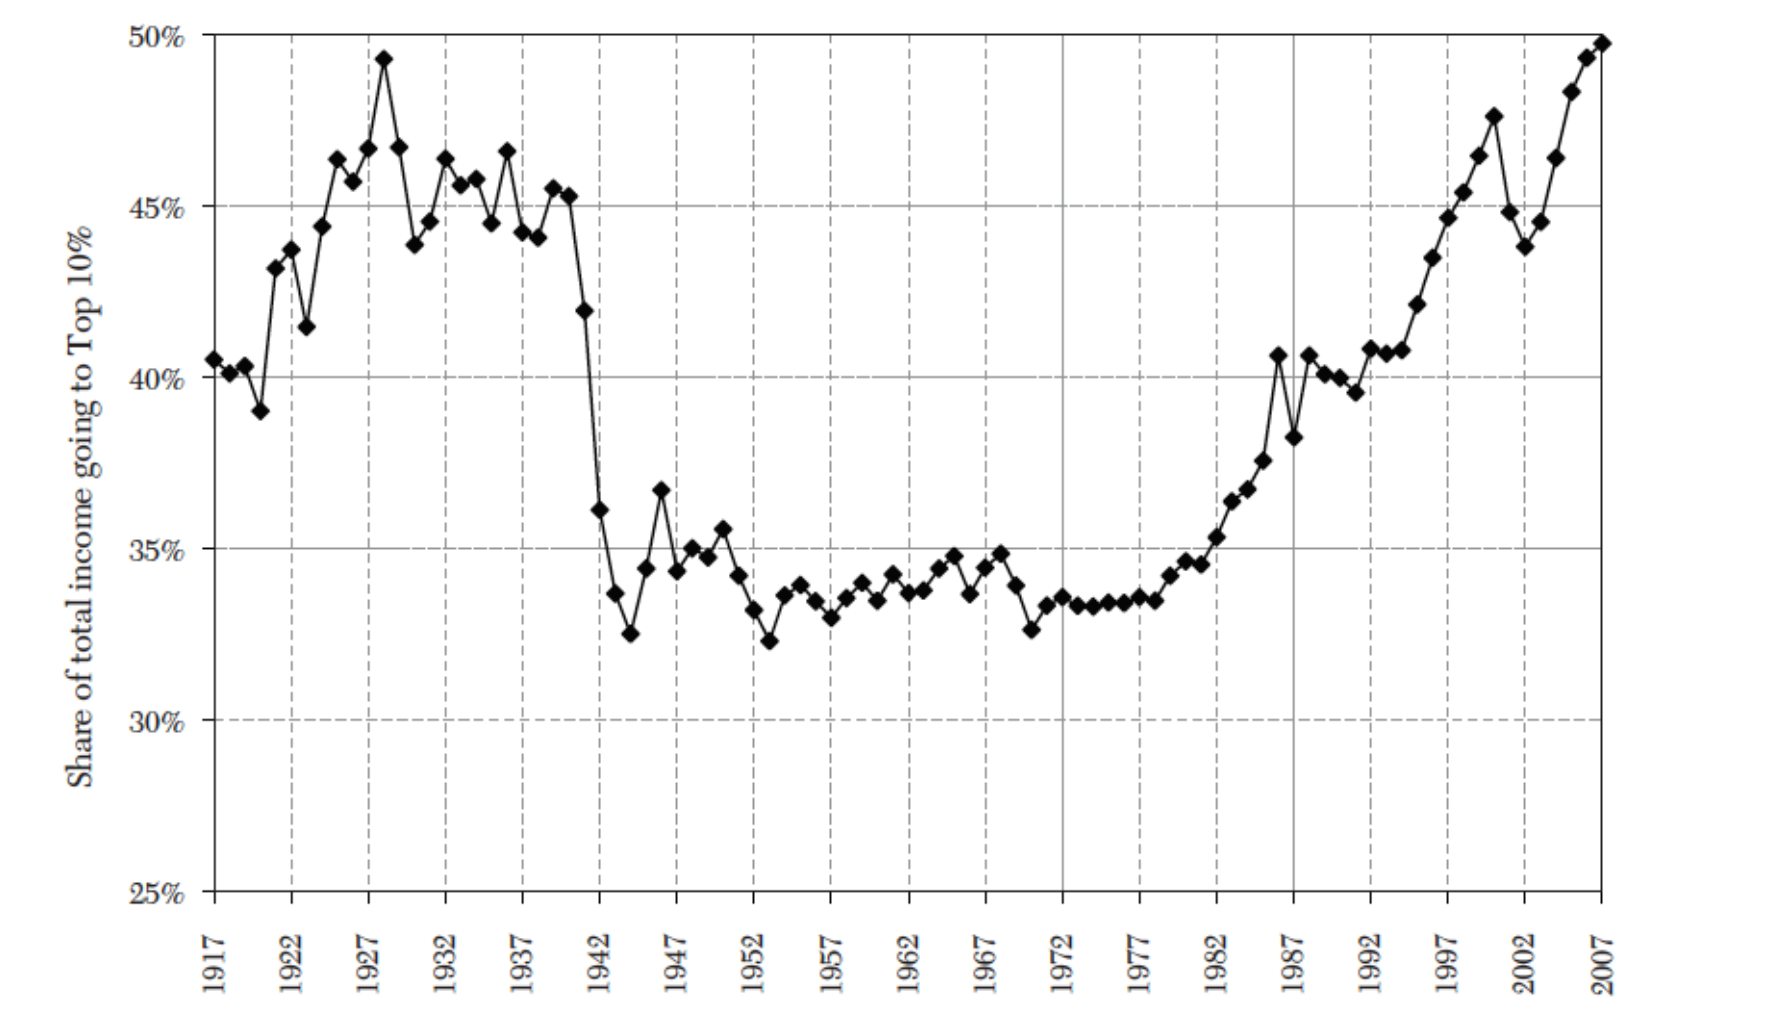
\includegraphics[width=4.5in]{images/ch13/13_inequality_1.png}
            \caption{The Top Decile Income Share in the United States, 1917–2007 (\cite{atkinson_top_2011})}
        \end{figure}

        The income share increased the most for the top percentile:

        \begin{figure}[H]
            \centering
            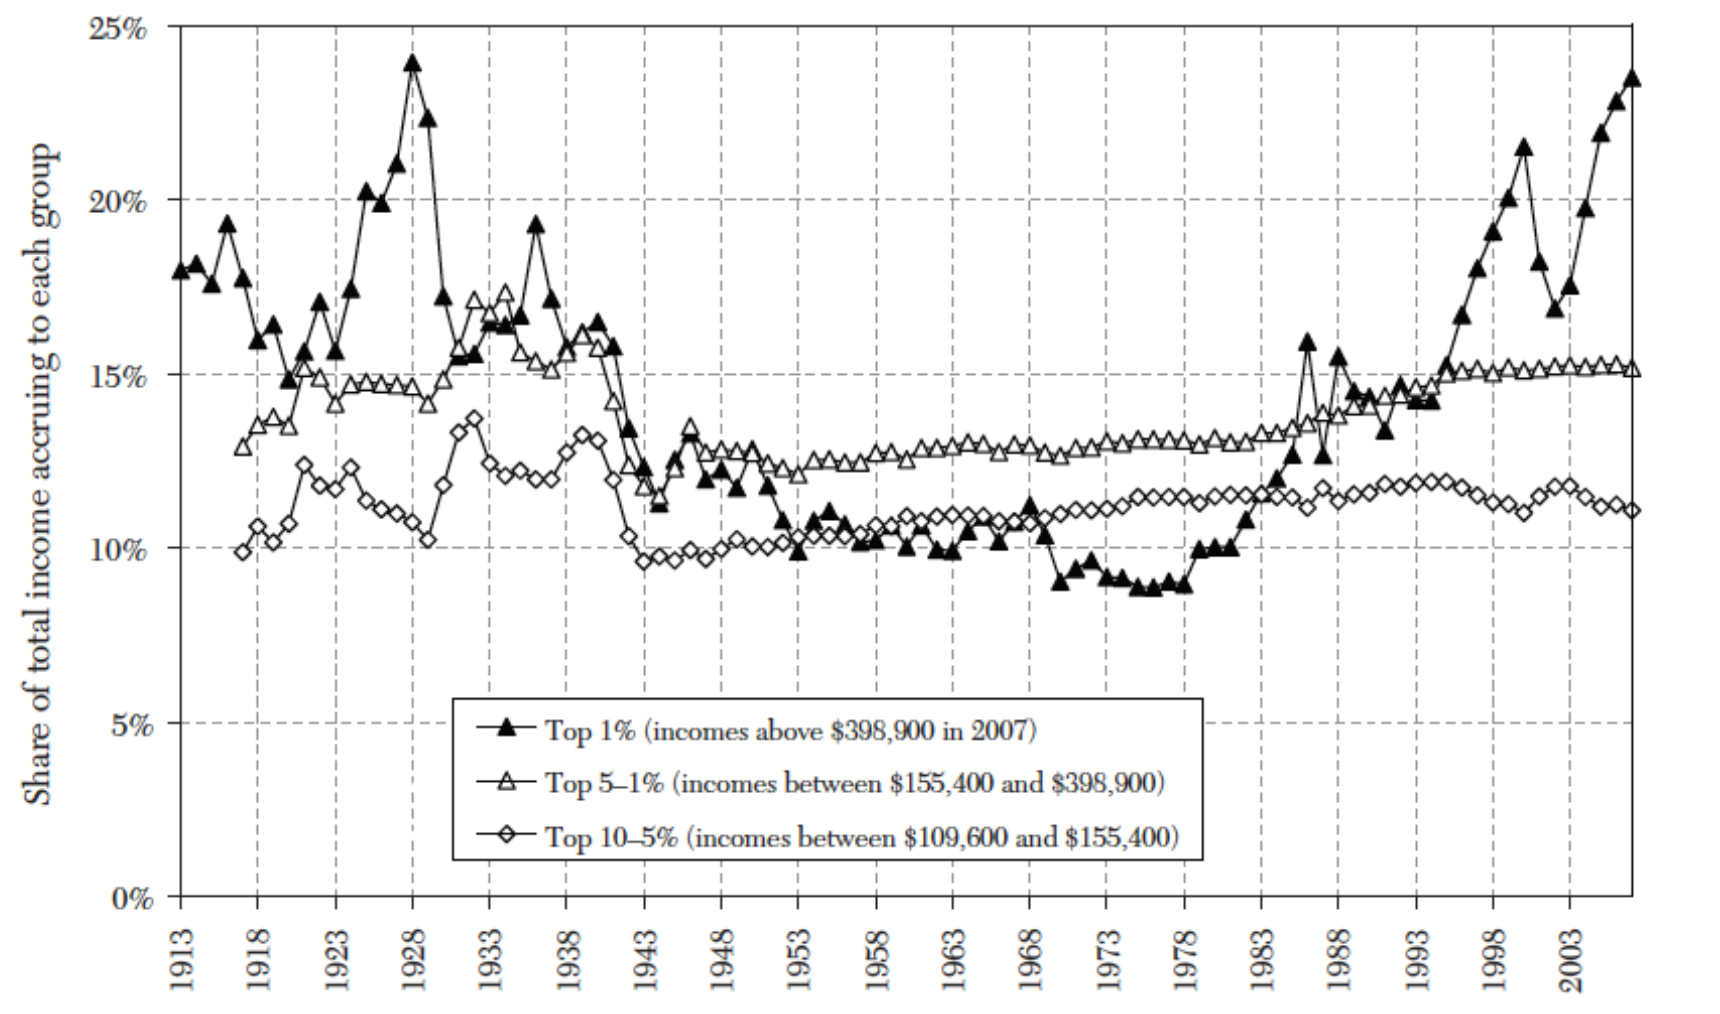
\includegraphics[width=4.5in]{images/ch13/13_inequality_2.png}
            \caption{Decomposing the Top Decile US Income Share into three Groups, 1913–2007 (\cite{atkinson_top_2011})}
        \end{figure}

        Meanwhile, the income gap between different educational groups also increased:

        \begin{figure}[H]
            \centering
            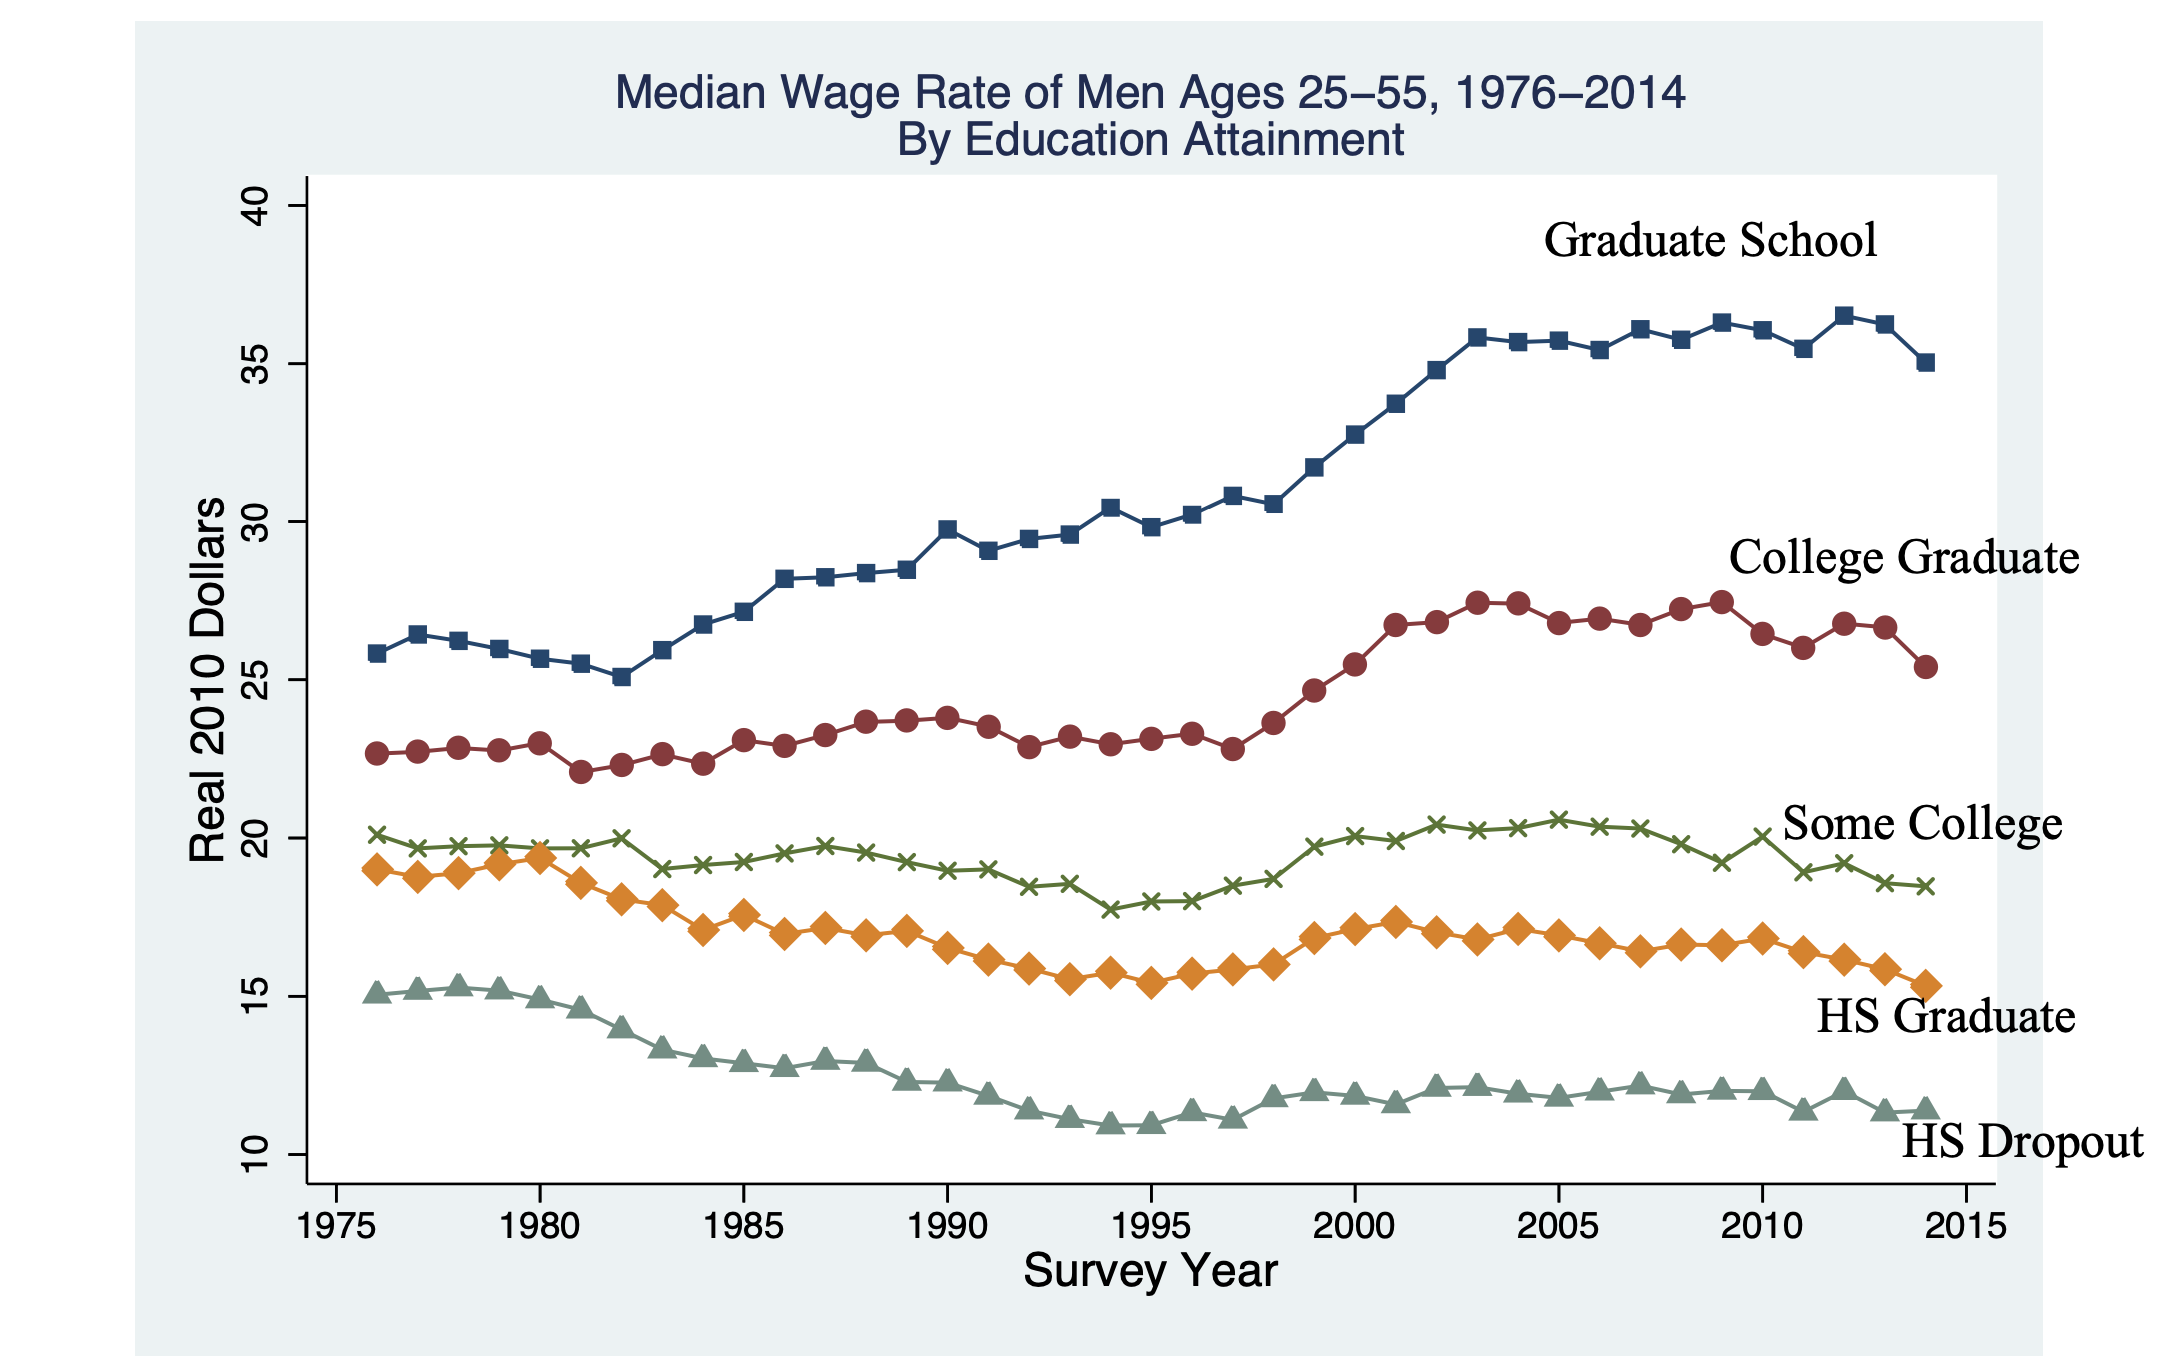
\includegraphics[width=4.5in]{images/ch13/13_inequality_3.png}
            \caption{Median Wage Rate of Men Ages 25-55, 1976-2014 (\cite{blundell_income_2018})}
        \end{figure}

\section{Introduction to Tax System}

    \subsection{Example Tax and Benefit Systems}

        \begin{figure}[H]
            \centering
            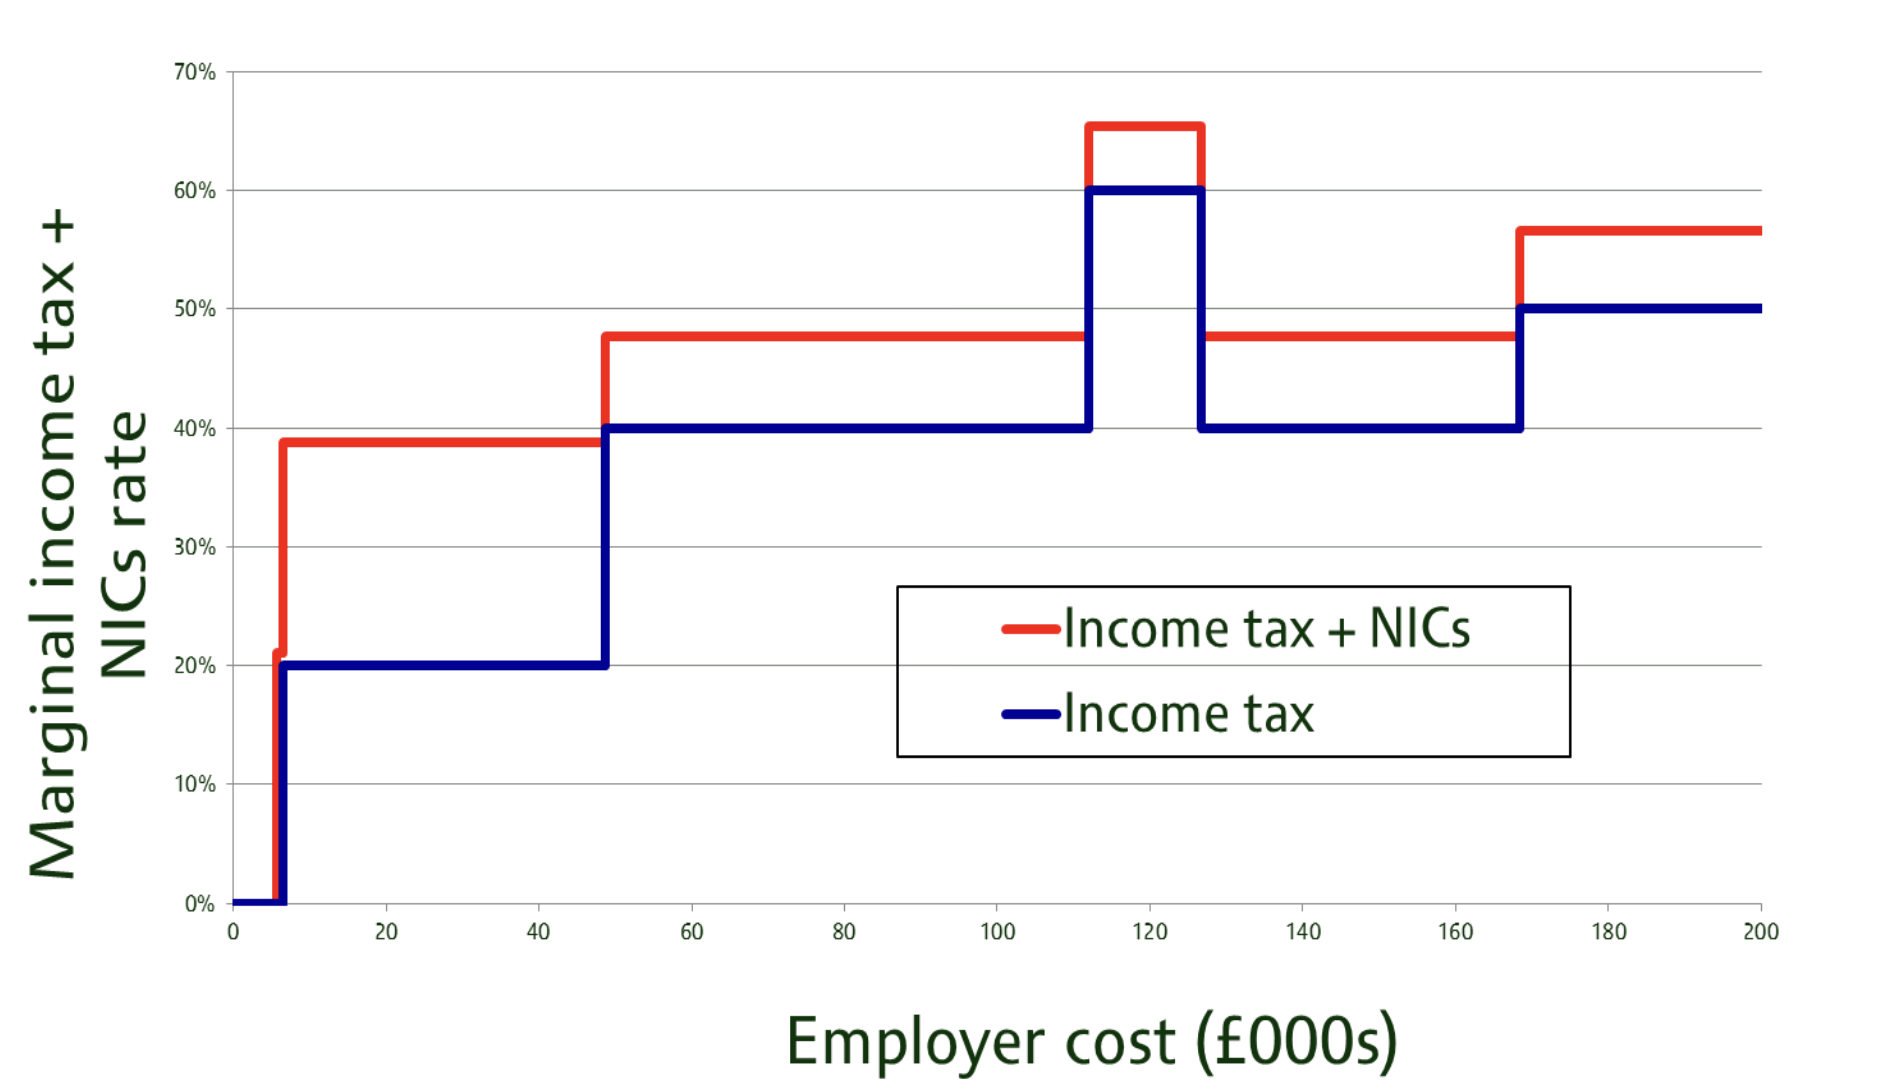
\includegraphics[width=4.5in]{images/ch13/13_taxscheme_1.png}
            \caption{Income Tax Schedule for Those Aged Under 65, UK 2010-11 (Mirrlees Review, 2011)}
        \end{figure}

        And the tax rate could be different for different sources of income:
        
        \begin{figure}[H]
            \centering
            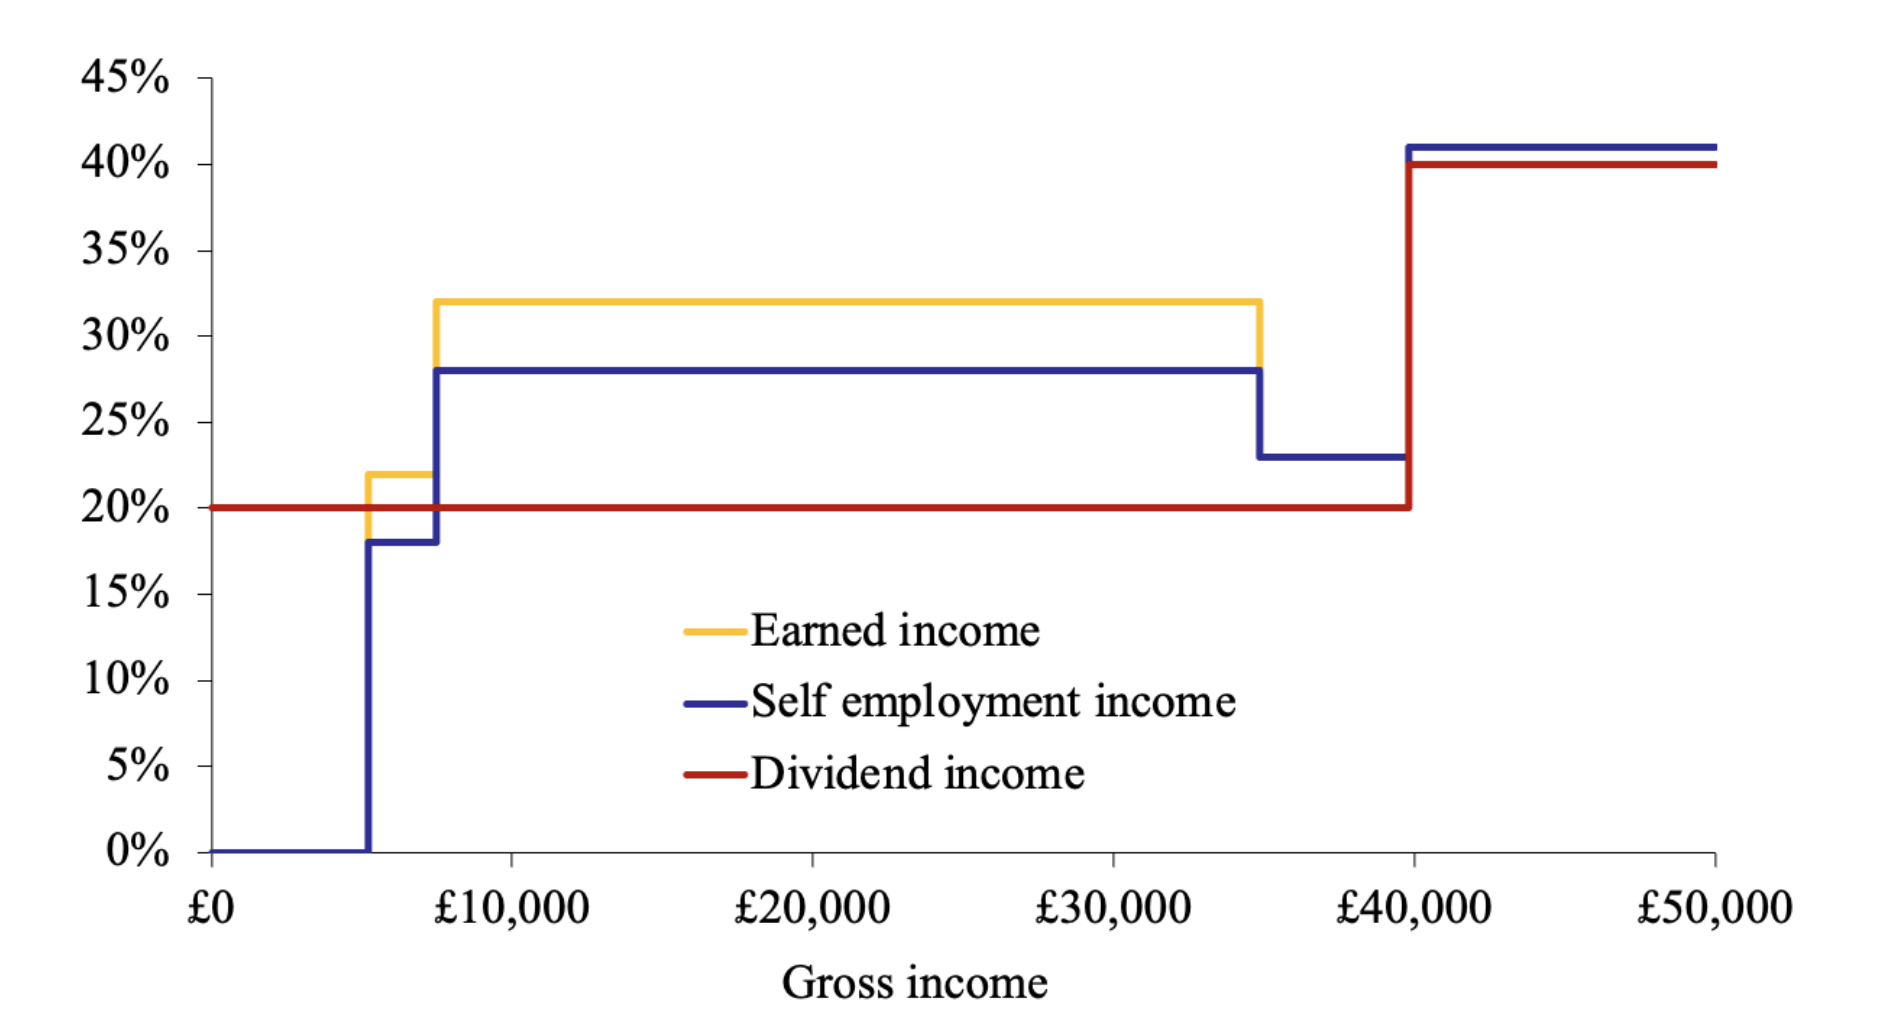
\includegraphics[width=4.5in]{images/ch13/13_taxscheme_2.png}
            \caption{Income Tax Schedule by Sources of Income for Those Aged Under 65, UK 2010-11 (Mirrlees Review, 2011)}
        \end{figure}

        \begin{figure}[H]
            \centering
            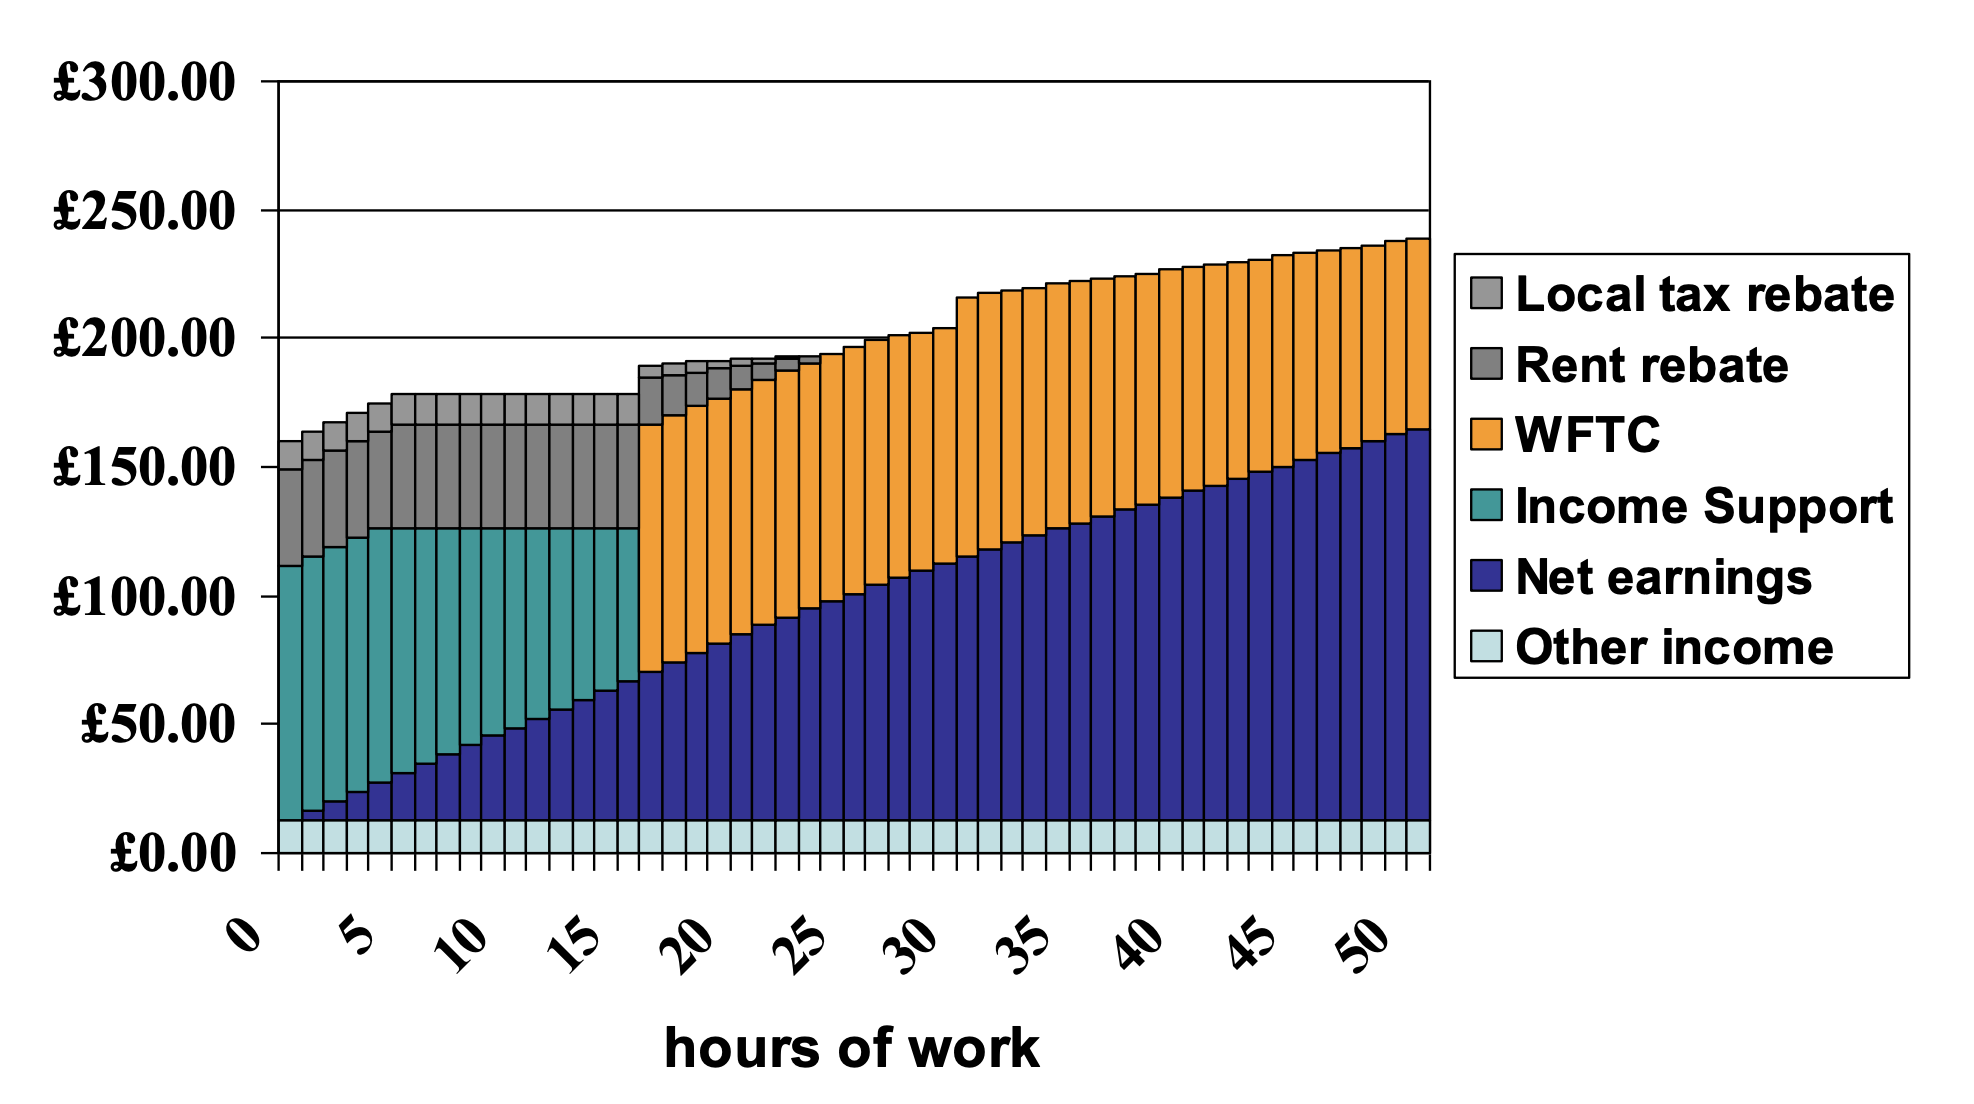
\includegraphics[width=4.5in]{images/ch13/13_taxscheme_3.png}
            \caption{Budget Constraint for Single Parent in UK}
        \end{figure}
    
    \subsection{Measuring Effective Tax Rates}

        The measurement of effective tax rates should:
        \begin{itemize}
            \item incorporate complete tax and transfer system
            \item consider both intensive and extensive margins
            \item account for earned income tax credits
        \end{itemize}

        \subsubsection{Effective Marginal Tax Rate (MTR)}

            The \emphb{Effective Marginal Tax Rate (MTR)} is the proportion of an \textsterling 1 of \empha{extra earning} retained in the tax and benefit system. This includes all employer taxes and contributions as well as the full set of taxes and benefits.
            
        \subsubsection{Participation Tax Rates (PTR)}

            The \emphb{Participation Tax Rates (PTR)} is the net loss, through taxes and benefits, of earnings in work \empha{relative to being out of work}. Typically, we assume a person works full-time when calculating PTR.

    \subsection{General Form of Earned Income Tax Credits (EITC)}

        \subsubsection{Overview of EITC}

        Definition of EITC: A subsidy given to low-income households in return for labour force participation.

        Goals of EITC:
        \begin{itemize}
            \item To increase worker welfare
            \item To offset high MTR and PTR created by income support, rent, and housing benefit schemes
        \end{itemize}

        Some features of EITC:
        \begin{itemize}
            \item Kinked benefits: credit depends on earnings and number of children, and there are 3 sections:
            \begin{enumerate}
                \item Phase-in: credit is flat percentage of earned income or jumps at minimum hours threshold ($MTR<0$)
                \item Flat range: receive maximum credit ($MTR=0$)
                \item Phase-out: credit is phased out at a flat rate ($MTR>0$); in the UK, the phase-out region in non-linear to encourage full-time work
            \end{enumerate}
            \item Credit is based on family earnings and is typically increasing in the number of children
            \item An individual must be participating the labour force to receive EITC (and subject to a minimal working hours eligibility constraint in the UK, which varies with family strucutres)
        \end{itemize}

        \subsubsection{EITC in U.S.}
        
            \begin{figure}[H]
                \centering
                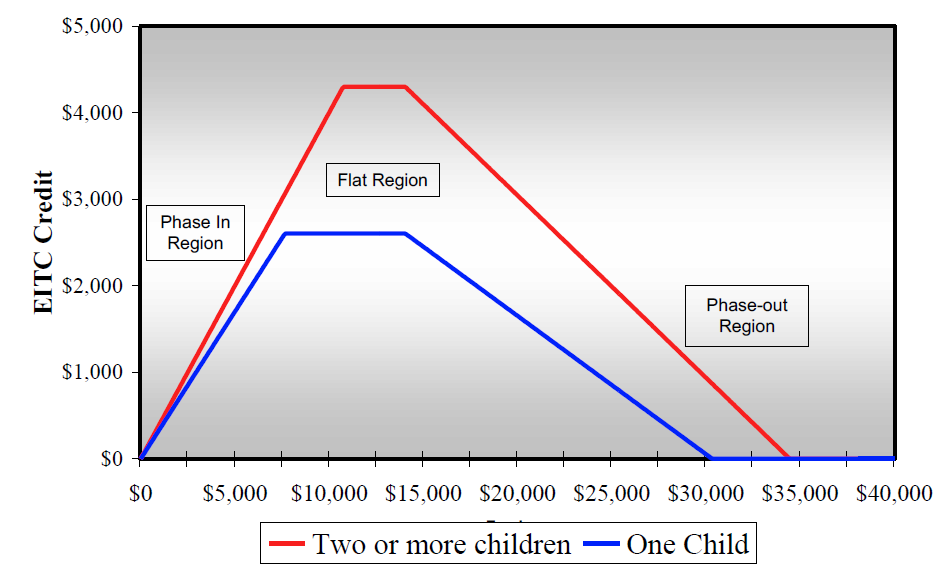
\includegraphics[width=4in]{images/ch13/13_US_EITC_1.png}
                \caption{The EITC Schedule in US}
            \end{figure}
            The US EITC schedule provides larger credit and covers higher earners for families with two or more children.
    
            \begin{figure}[H]
                \centering
                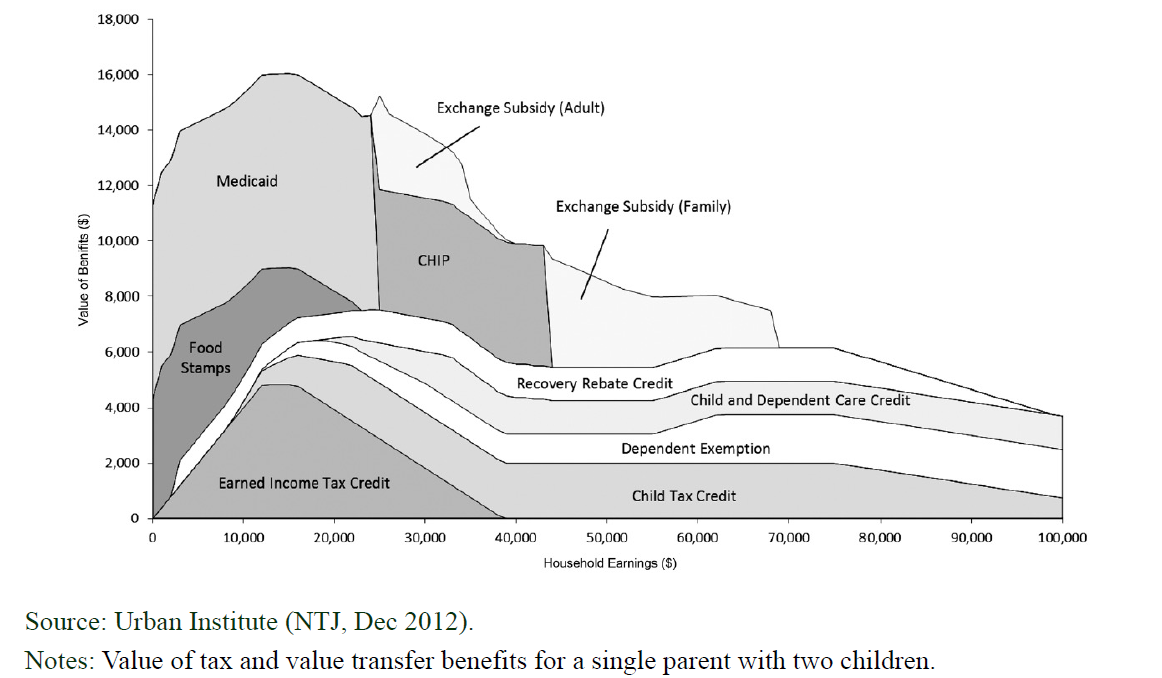
\includegraphics[width=5in]{images/ch13/13_US_Tax_and_trans.png}
                \caption{Universally Available Tax and Transfer Benefits in US}
            \end{figure}
    
            \begin{figure}[H]
                \centering
                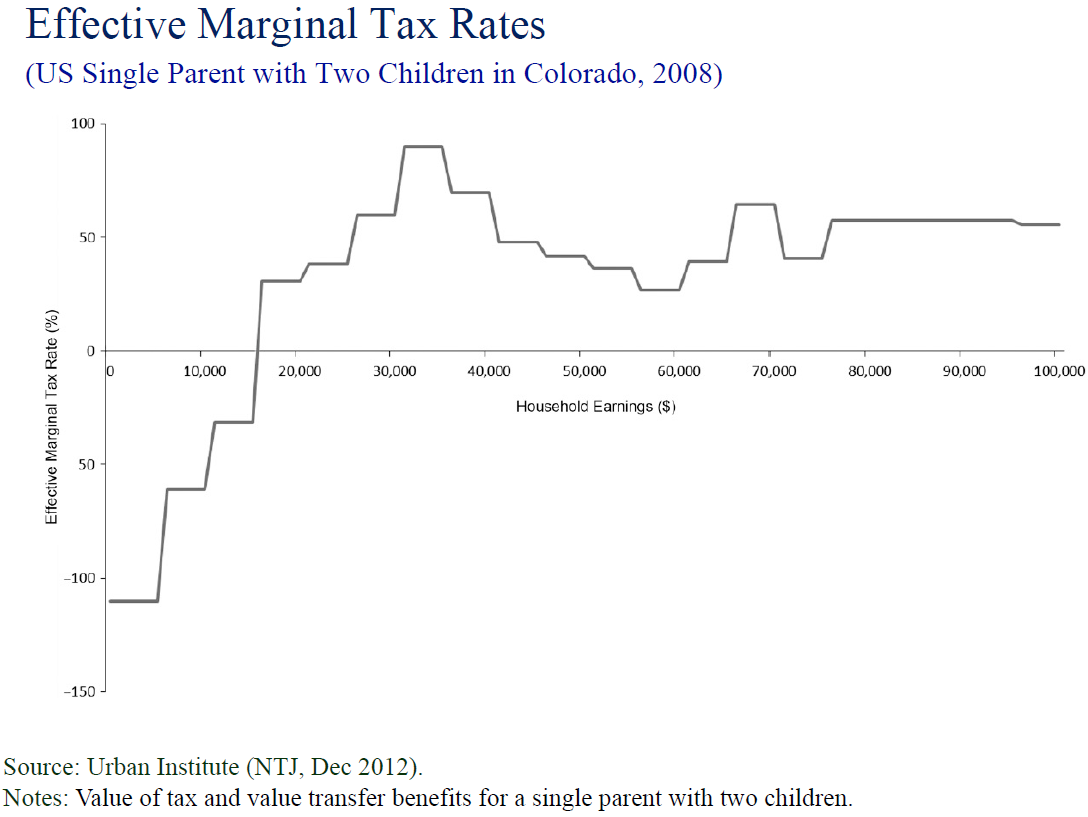
\includegraphics[width=4in]{images/ch13/13_US_MTR.png}
                \caption{US Effective Marginal Tax Rates (MTR)}
            \end{figure}
            When income is low, MTR is largely negative, providing big subsidies. As income increases, MTR rises and stabilises at around 50\%.

        \subsubsection{Working Families Tax Credit (WFTC) in the UK}

            Particular features of UK Working Families Tax Credit:
            \begin{itemize}
                \item Hours of work condition:
                \begin{itemize}
                    \item There is a minimum hours rule -- 16 hours per week
                    \item An additional hours-contingent payment at 30 hours    
                \end{itemize}
                \item Family eligibility -- adult credit plus amounts for each child in full time education or younger
                \item Income eligibility -- family net income has to be below a certain threshold
            \end{itemize}

            \begin{figure}[H]
                \centering
                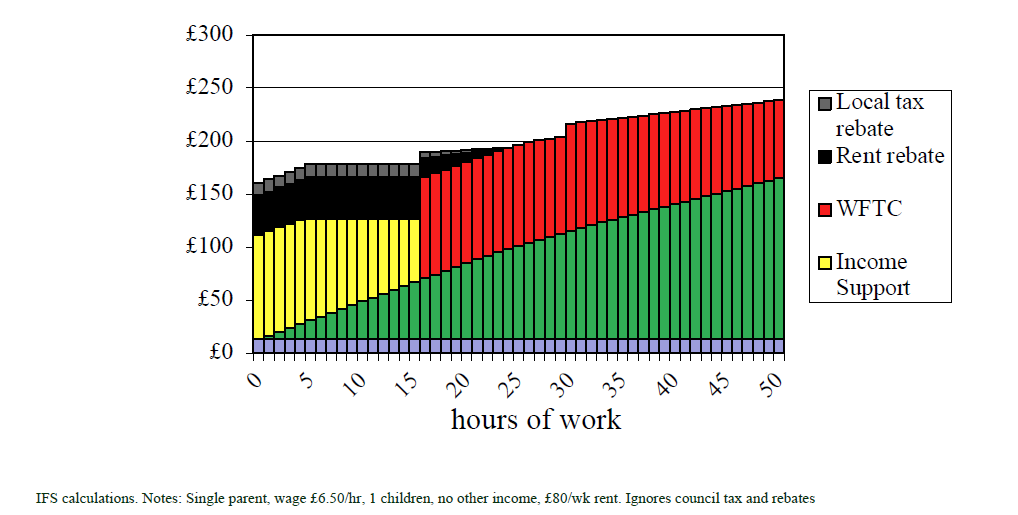
\includegraphics[width=5.5in]{images/ch13/13_UK_Tax_and_trans.png}
                \caption{The Interaction Between Taxes, Tax Credits and Benefits in UK}
            \end{figure}

            \begin{figure}[H]
                \centering
                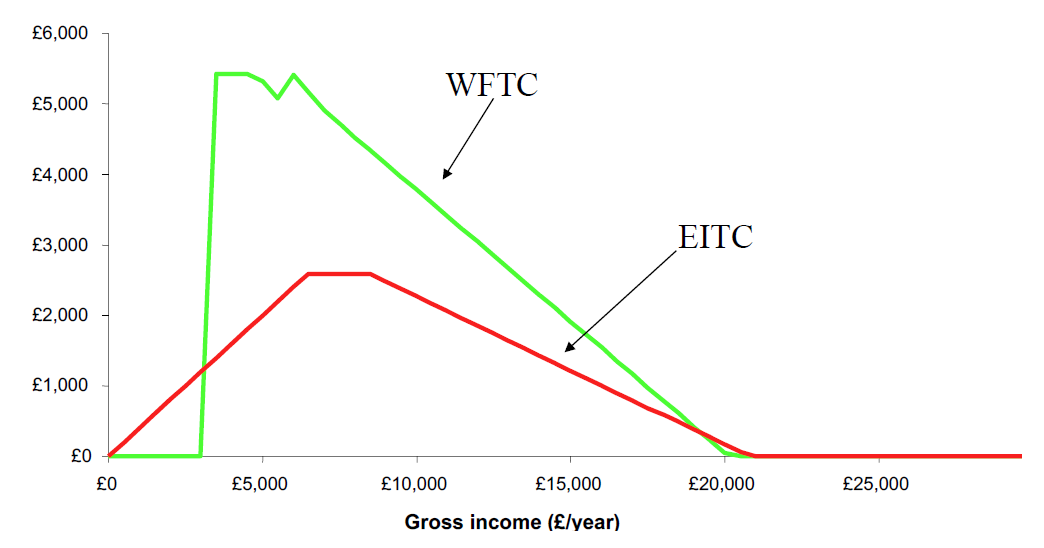
\includegraphics[width=4in]{images/ch13/13_USUK_credit_compare.png}
                \caption{The UK and US Tax Credit System Compared}
            \end{figure}

        \subsubsection{Why are EITCs Typically Directed to Working Age Adults with Children?}

            \begin{itemize}
                \item To promote child welfare\\
                Supporting a child in the early life could lead to higher human capital in the long run, promoting inter-generational welfare
                \item To encourage parents with low skills/income to re-enter the labour market\\
                Income tax credits can be interpreted as a boost of wages for those who are in low-wage professions, making parents less likely to stay at home (especially effective for working mothers due to their high labour supply elasticity)
                \item To reduce the cost of childcare\\
                With more disposable income, parents can spend more money instead of time on childcare, and hence increase their working time
            \end{itemize}

        \subsubsection{How EITCs Attempt to Balance the Dual Objectives of Work Incentives with Redistribution?}

            In short, EITC schemes are designed to transfer incomes to households in the lower end of the income distribution while provide them with incentives to stay in the labour force.

            An Case Study of the UK:
            \begin{itemize}
                \item Study the policy shift: family credits $\to$ working family tax credits (WFTC)
                    \begin{figure}[H]
                        \centering
                        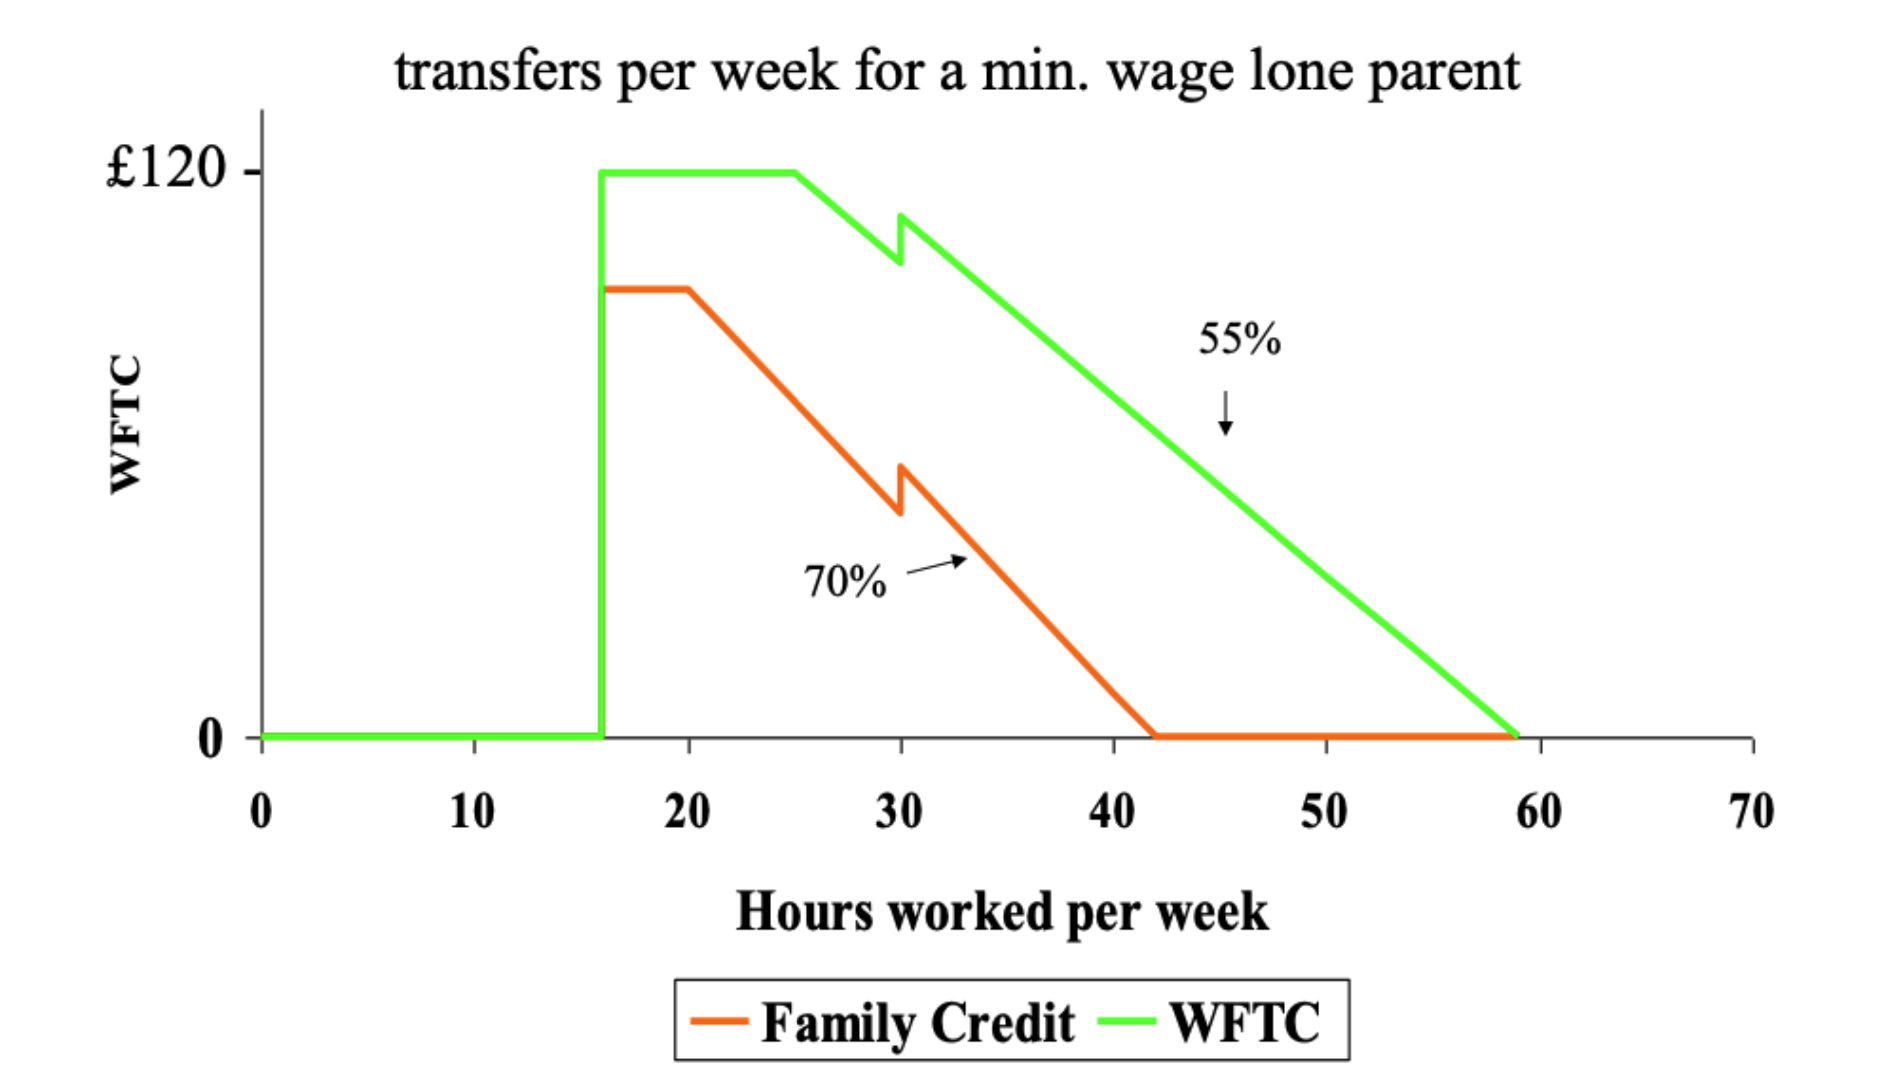
\includegraphics[width=4in]{images/ch13/13_uk_casestudy_1.png}
                    \end{figure}
                \item Distributional effect (\cite{dilnot_family_1999}):
                    \begin{figure}[H]
                        \centering
                        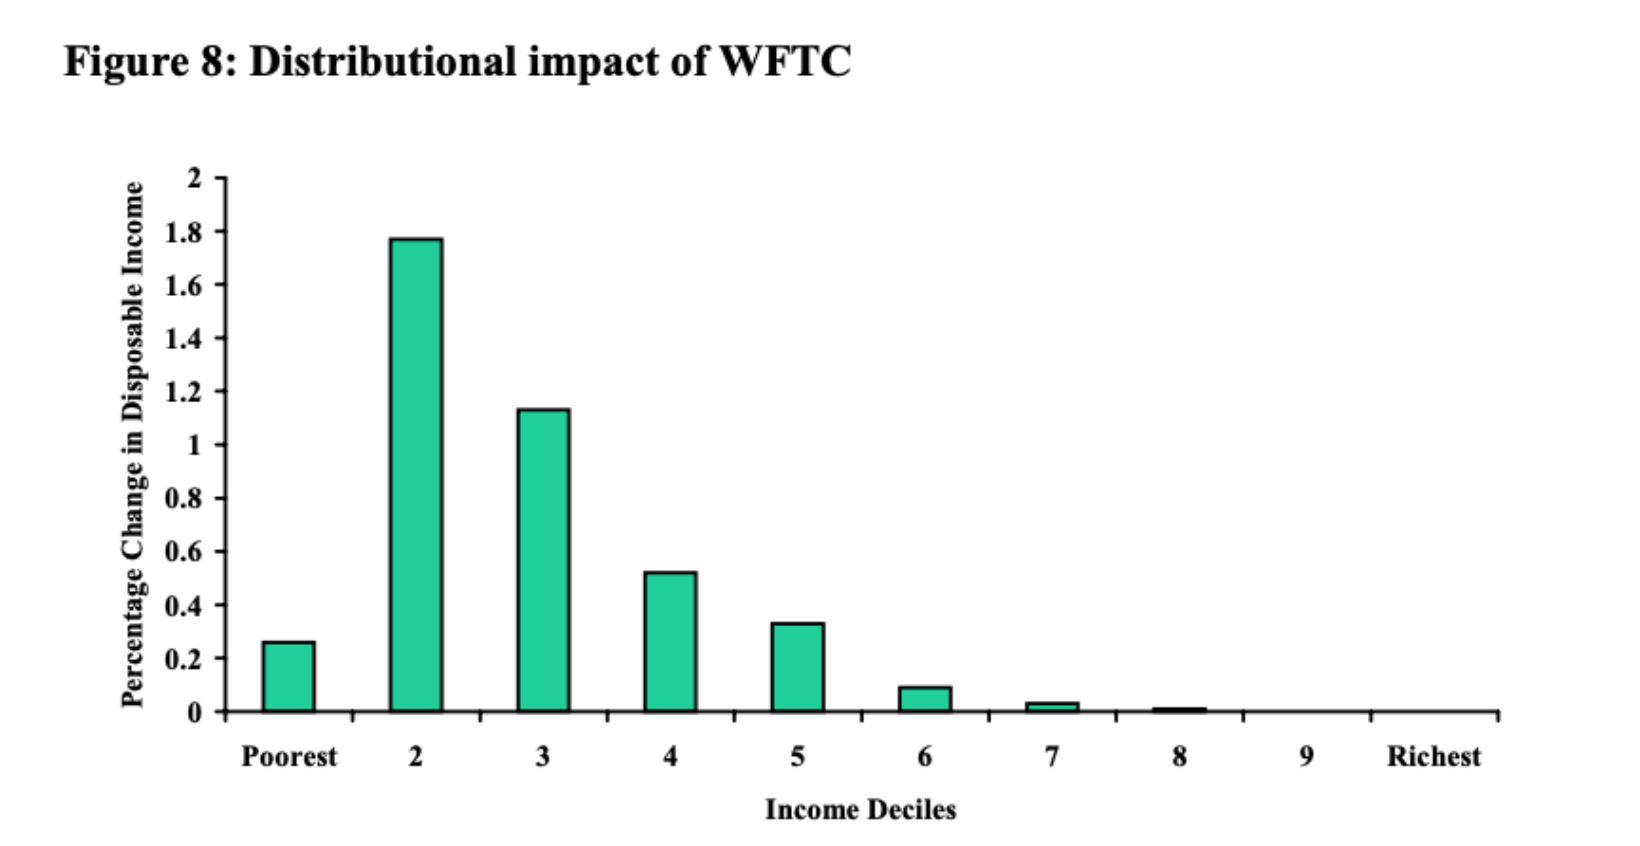
\includegraphics[width=4in]{images/ch13/13_uk_casestudy_2.png}
                    \end{figure}
                \item Incentive effect: EITCs shifts up both the initial wage and the budget constraint and hence induces people to both participate in the labour market and work more (if substitution effects dominate). \cite{blundell_labour_2000} used simulation to show that both LFPR and hours worked increase for single parents earning median hourly wage:
                    \begin{figure}[H]
                        \centering
                        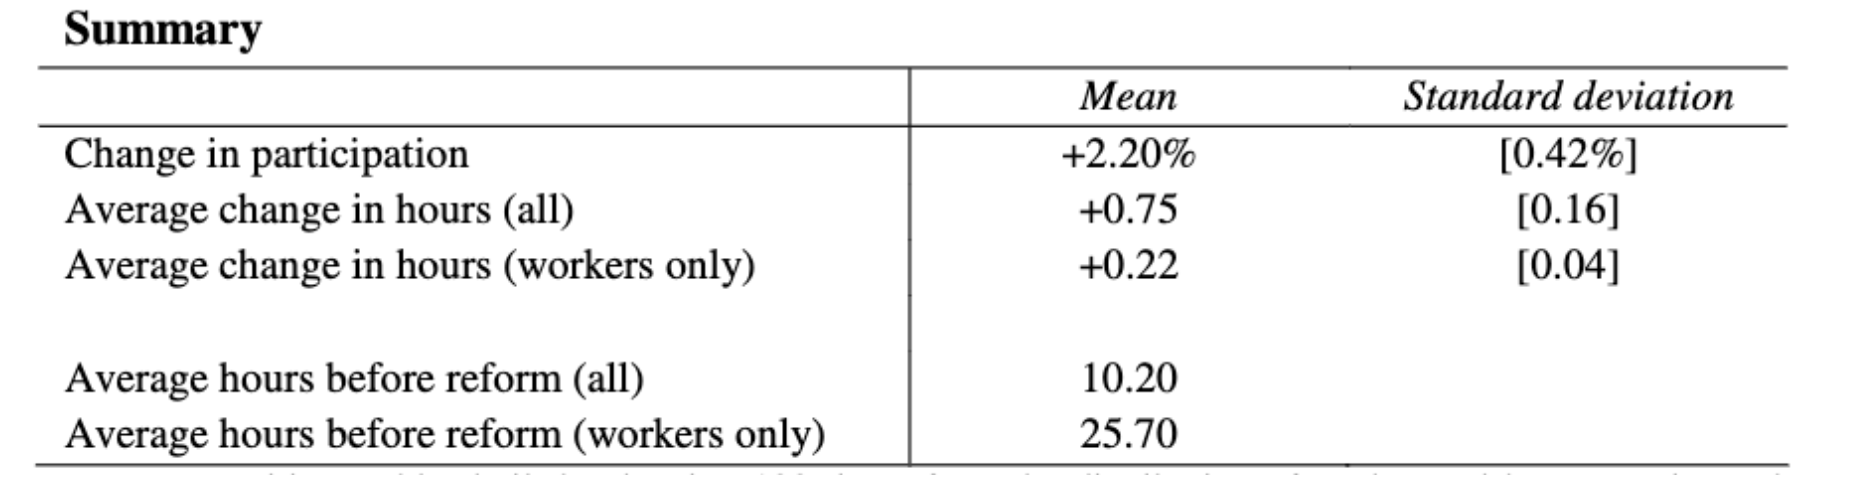
\includegraphics[width=4in]{images/ch13/13_uk_casestudy_3.png}
                    \end{figure}
            \end{itemize}

        \subsubsection{Bunching at Tax Kinks and the EITC}

            \begin{figure}[H]
                \centering
                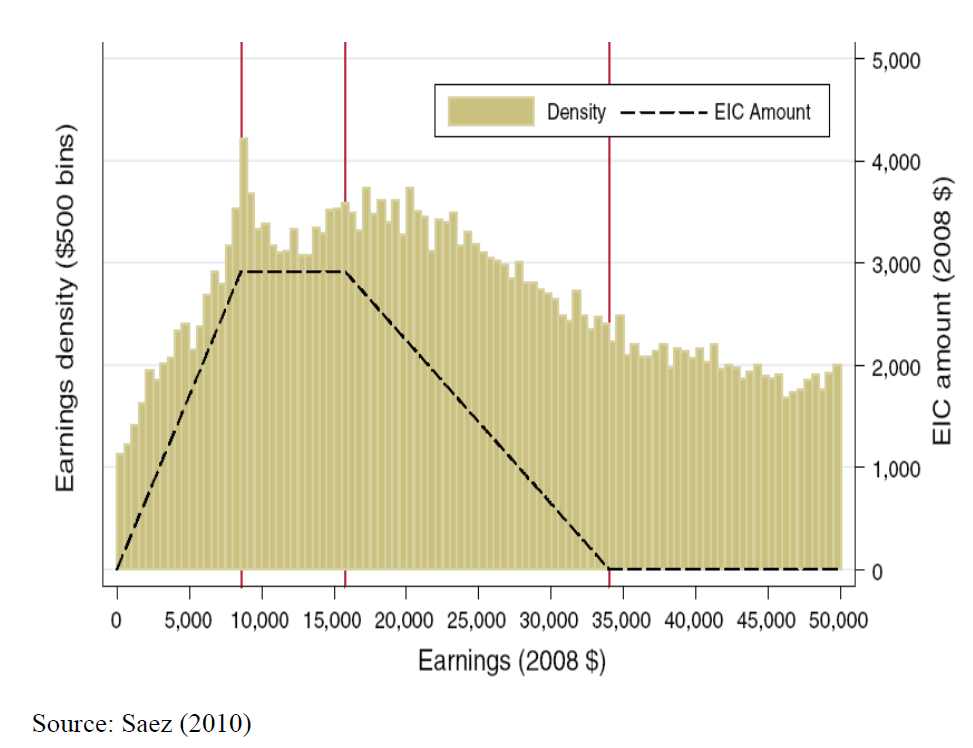
\includegraphics[width=4in]{images/ch13/US_Bunching_EITC_1.png}
                \caption{Bunching at Tax Kinks and the EITC -- One Child Families, U.S.}
            \end{figure}

            If people are optimising, they should be clustered at kinks (bunching) and avoid gaps. Here, we observe some extents of bunching at the first kink, but not at the second one.
        

\section{$\star$ Optimal Tax Design on the Top Earners}\label{sec:optimal_top_tax}

    \subsection{Introduction}

        \cite{mirrlees_theory_1971} views taxation as an \emphb{information problem}. The government only observes whether people work and how much they earn. The government cannot observe effort -- it cannot distinguish a high ability person working few hours from a low ability person working a lot.

        In this framework, a tax schedule is chosen to \empha{maximise social welfare} and \empha{raise a required amount of revenue}. It needs to reach a \empha{balance between redistributive aims and effort incentives}. If it taxes high-ability people too much, they may choose to supply less effort. Thus, we need good estimates of labour supply elasticises.

    \subsection{Three Impacts on Social Welfare}\label{sec:optimal_top_tax_impacts}

        \subsubsection{Setup}

        \begin{itemize}
            \item Consider a reform that changes the top tax rate $\tau$ by a small amount $d\tau$.
            \item Let $z$ be the earned income being considered for taxation
            \item The top income bracket begins at income $z^*$
            \item There are $N$ taxpayers in the top bracket
        \end{itemize}
        
        \subsubsection{Mechanical Effect on Tax Revenue ($dM$)}

            With no behaviour response, an increase of the top rate will increase government revenue. This is beneficial to society, as the revenue can be used for government spending or higher transfers.

            Mathematically:

            \begin{equation}
                dM = N \times (z-z^*) \times d\tau > 0
                \label{eqn:tax_top_TR}
            \end{equation}

        \subsubsection{Behaviour Response on Tax Revenue ($dB$)}

            Higher top rate can also induce top bracket taxpayers to reduce their hours of working (substitution effect) and decrease their earnings. This is a cost to society as tax revenue will fall.

            Note that there will be no change for taxpayers in other tax bracket because nothing has changed for them.

            Mathematically, this behavioural effect depends on the \emphb{elasticity of earnings with respect to the net of tax rate ($1-\tau$)}

            \begin{equation*}
                e = \frac{d z}{d (1-\tau)} \frac{1-\tau}{z} = -\frac{d z}{d \tau} \frac{1-\tau}{z}
            \end{equation*}
            
            \begin{equation*}
                dz = -e \times z \times \frac{d\tau}{1-\tau}
            \end{equation*}

            Hence, tax revenue will be reduced by:

            \begin{equation}
                dB = - N \times e \times z \times d\tau \times \frac{\tau}{1-\tau}
                \label{eqn:tax_top_BR}
            \end{equation}

        \subsubsection{Welfare Effect ($dW$)}

            Any increase in the top rate will reduce the welfare of top bracket taxpayers. This is a loss to society.

            If the government values redistribution, then the marginal ``value'' of income will be small after the income goes above certain level. In the limit, when a taxpayer's income is extremely high, the welfare effect will be negligible relative the the mechanical effect on tax revenue.

            The government gives a value of $g$ to an extra \textsterling 1 earned by top tax bracket taxpayer. This will be strictly less than 1 because the weighted sum of welfare weights in unity.

            Thus, the welfare effect of higher marginal tax rate on incomes above $z^*$ is:

            \begin{equation}
                dW = -g \times N \times (z-z^*) \times d\tau < 0
                \label{eqn:tax_top_WE}
            \end{equation}

    \subsection{The Choice of the Top Tax Rate}

        \subsubsection{Optimum}

            Summing up the three effects (equation \ref{eqn:tax_top_TR}, \ref{eqn:tax_top_BR}, and \ref{eqn:tax_top_WE}). The overall effect of a small change in top rate ($d\tau$) is:
    
            \begin{equation*}
                dM + dB + dW = Nd\tau (z-z^*) \left( 1-g-ea \frac{\tau}{1-\tau} \right)
            \end{equation*}
    
            where $a= \frac{z}{z-z^*}$ is the \emphb{Pareto parameter}: higher $a$ indicates a thinner tail.
    
            At optimum, this has to be zero:
    
            \begin{equation*}
                dM + dB + dW = Nd\tau (z-z^*) \left( 1-g-ea \frac{\tau}{1-\tau} \right) = 0
            \end{equation*}
    
            This can be simplified to:
    
            \begin{equation}
                \color{red}
                \tau^* = \frac{1-g}{1-g+ae}
            \end{equation}

        \subsubsection{Interpretation}

            There are some nice interpretations of this simple formula:
            \begin{itemize}
                \item Note that $a$ is a parameter of the upper tail of the Pareto distribution with pdf: $f(z)=\frac{C}{z^{1+a}}$
                \item \empha{If $g$ is approximately zero (low weight placed on high-earners / purely revenue maximising), then:}
                \begin{equation}
                \color{red}
                    \tau^* = \frac{1}{1+ae}
                \end{equation}
                This is very simply to calculate if we know the Pareto parameter $a$ and taxable income elasticity $e$
                \item Estimation of the Pareto parameter $a$ and taxable income elasticity $e$ is important
            \end{itemize}

            The next section explores the estimation of those two parameters. We will see that \empha{with estimated $a=1.67$ and $e=0.46$ (using DiD method), the revenue maximising tax rate for the top 1\% is aroun 56\%.}

        \subsection{Extension: The Choice of the Top Tax Rate with Migration Responses}

            In addition, individuals may respond to higher taxes by migrating to other countries. This is similar to an \emphb{extensive margin}.

            Denote the \emphb{migration elasticity} as $m$, and \empha{ignore distributional effects ($g$ is approximately zero: low weight placed on high-earners / purely revenue maximising)}.

            The optimal top tax rate will be:
            \begin{equation}
                \color{red}
                    \tau^* = \frac{1}{1+ae+m}
            \end{equation}

            By nature, the migration elasticity $m$ is hard to estimated, and there are discussions on whether it changes with the business cycle.

            Note that if the migration elasticity $m$ is high, governments need certain accordance to aviod "tax competitions."


    \section{Estimating the Pareto Parameter $a$ and Taxable Income Elasticity $e$}

        \subsection{Estimating the Pareto Parameter $a$}

            The Pareto parameter $a$ is easy to estimate -- we only need to fit the pdf curve with real world data.

            \begin{figure}[H]
                \centering
                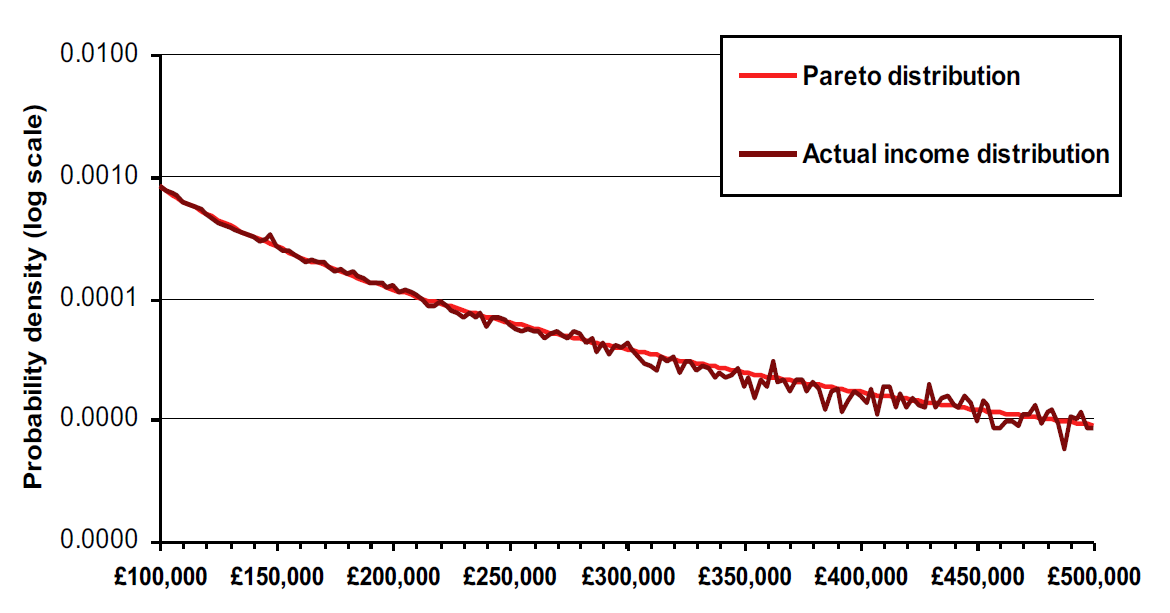
\includegraphics[width=4.5in]{images/ch13/13_UK_Pareto_para.png}
                \caption{Top Income Distribution in the UK}
            \end{figure}

            The Pareto parameter for the UK is quite accurately estimated to be 1.67.

            Note that Pareto distribution has no moments because its upper tail is not capped.

        \subsection{Measuring Response Elasticity: Overview}

            Measuring people's responsiveness with respect to a change in MTR is hard. Typically, researchers adopt 4 broad approaches:
            \begin{itemize}
                \item Randomised Control Trials (RCT)
                \item Quasi-experinments (DiD)
                \item Bunching Approaches
                \item Structual Approaches
            \end{itemize}

        \subsection{RCT: Canadian Self Sufficiency Program (SSP)}

            \subsubsection{Setup}

                Caveat: this RCT assesses workers at the lower end of the income distribution.

                The Canadian Self Sufficiency Program (SSP) is designed to answer: do financial incentives encourage work among low skilled lone parents?

                To encourage employment among welfare recipients, especially single parents on welfare, randomly selected participants are treated as following:
                \begin{itemize}
                    \item A tax credit equals to 50\% of earnings is provided (on earnings up to \$ 36000)
                    \item Work at least 30 hours per week to be eligible
                \end{itemize}

                The budget constraints of treated/control groups are:
                
                \begin{figure}[H]
                    \centering
                    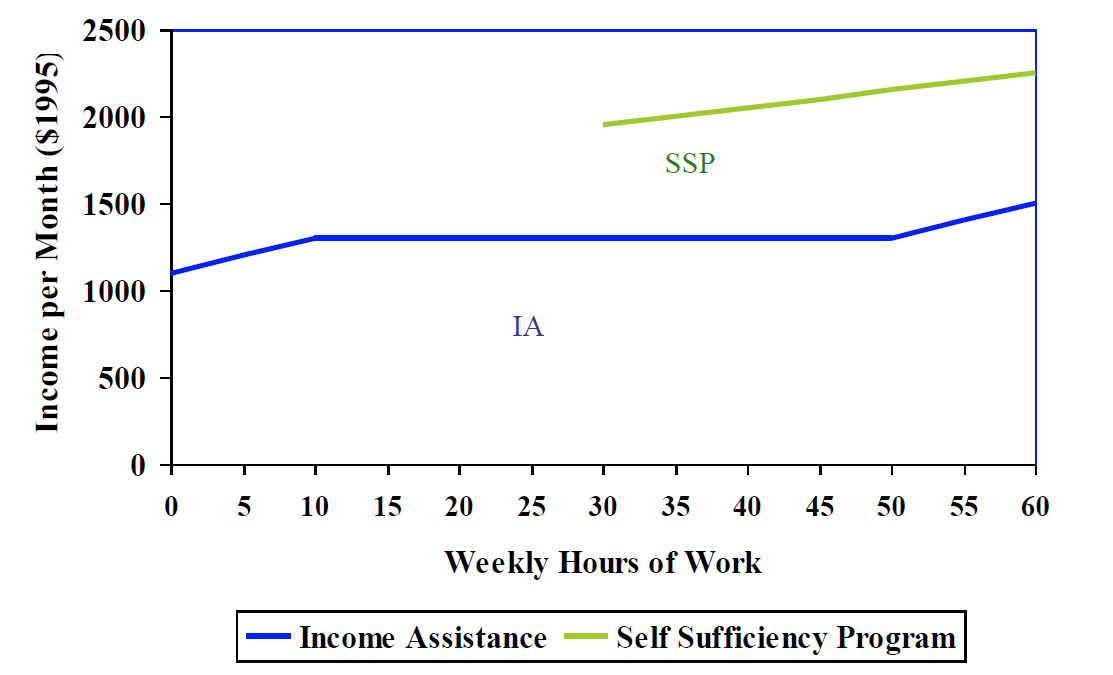
\includegraphics[width=4.5in]{images/ch13/13_SSP_1.png}
                    \caption{Budget Constraint for a Single Parent on Minimum Wage}
                \end{figure}

            \subsubsection{Results}

                \begin{figure}[H]
                    \centering
                    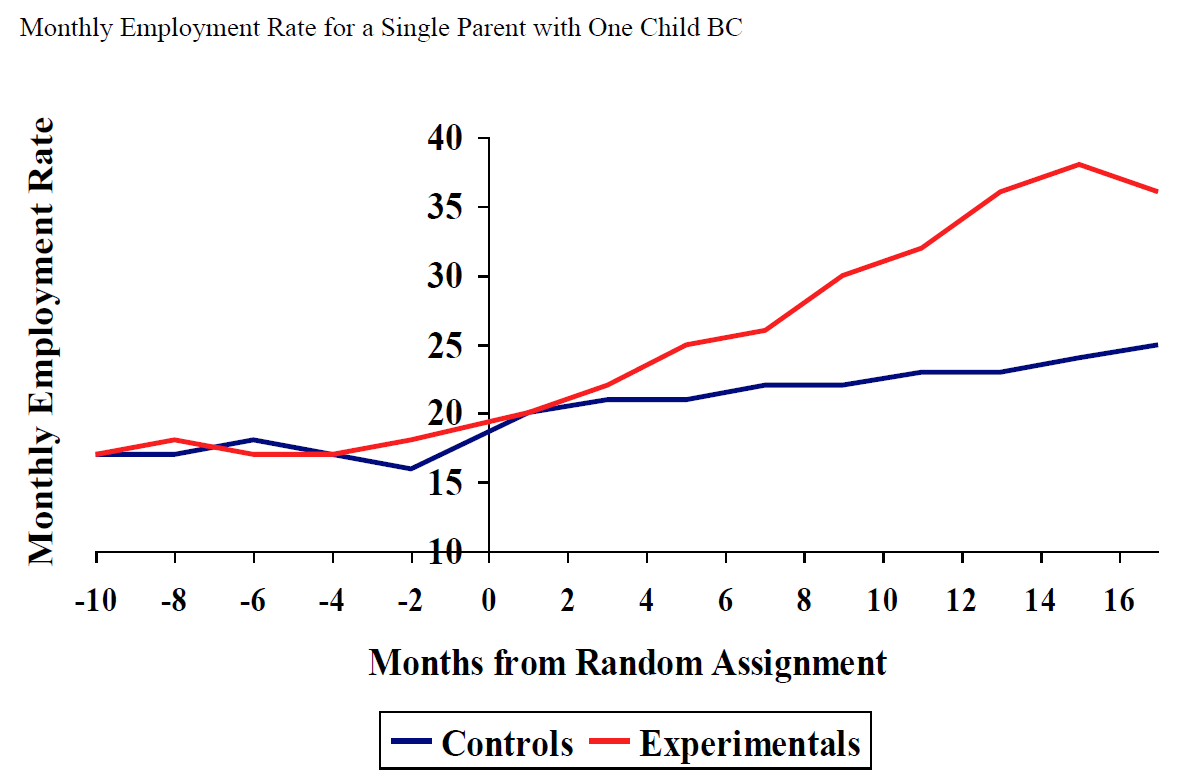
\includegraphics[width=4.5in]{images/ch13/13_SSP_2.png}
                    \caption{Monthly Employment Rate for a Single Parent with One Child}
                \end{figure}

                The treatment/control groups are well balanced before the treatment. After treatment, we observe that the employment rate of participants with tax credits becomes significantly higher than the control group.

            \subsubsection{Caveat for RCTs in Social Science}

                Unlike in Medicine or Physics, RCTs in social science can never be perfect because we cannot generate a perfect placebo. There will always be some placebo or spillover effects.
                
        \subsection{Quasi-experiments (Diff-in-Diff)}

            \subsubsection{History of Top Tax Rates in the UK (\cite{brewer_means-testing_2010})}

                \begin{figure}[H]
                    \centering
                    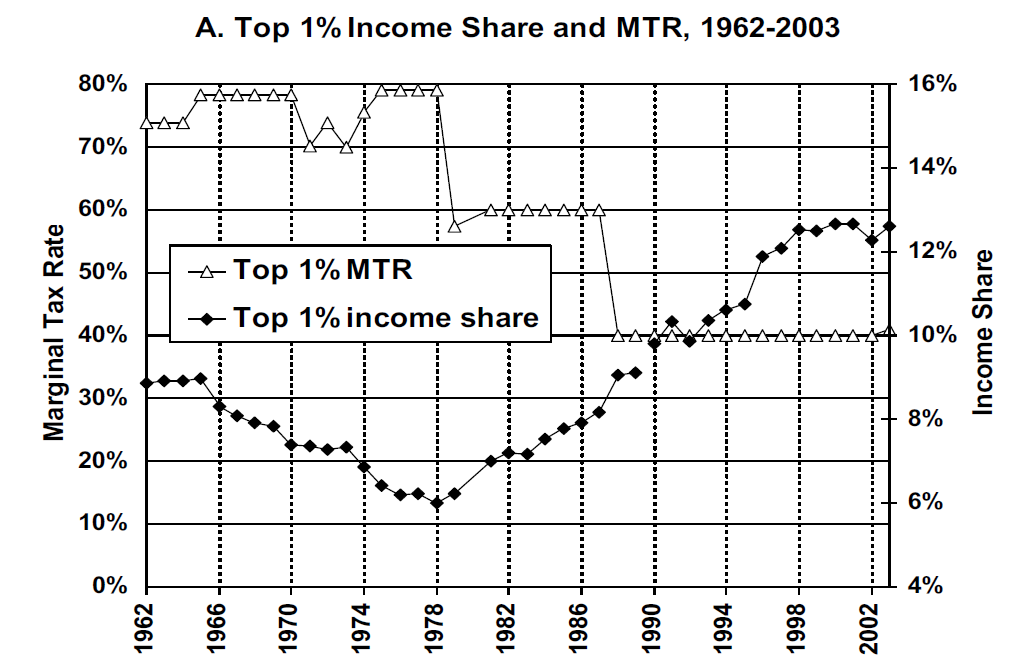
\includegraphics[width=4.5in]{images/ch13/13_DID_1.png}
                    \caption{Top 1\% Income Share and MTR, 1962-2003}
                \end{figure}

                From 1978 to 1990, the MTR of the top 1\% income earners decreases dramatically.
                    
                \begin{figure}[H]
                    \centering
                    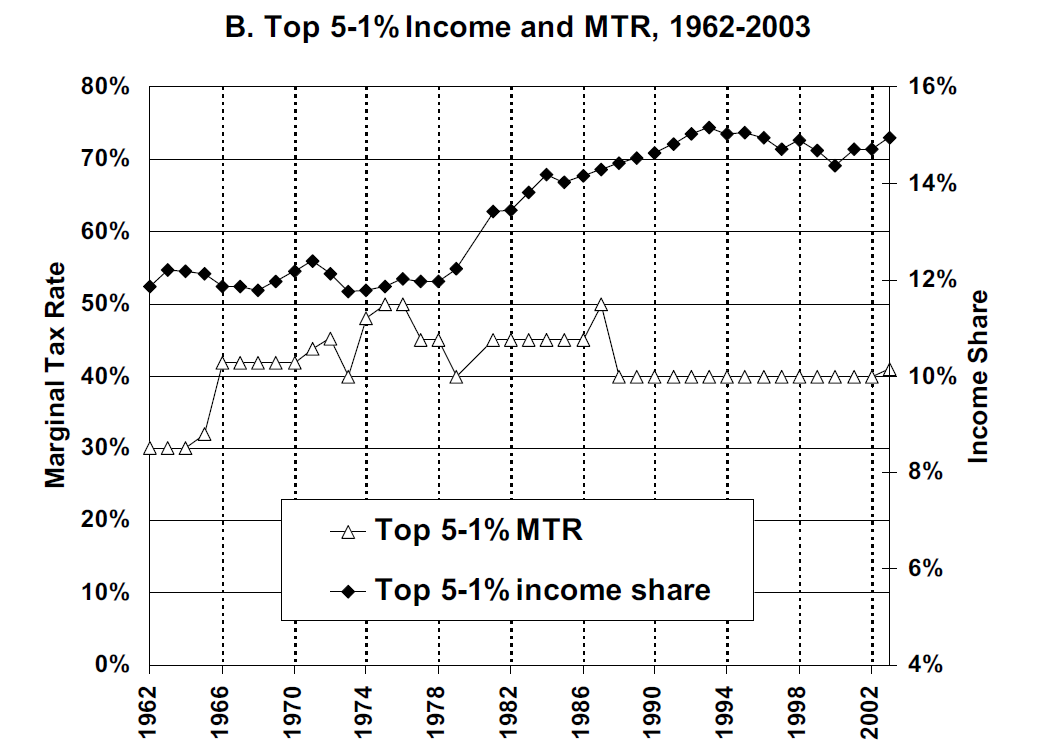
\includegraphics[width=4.5in]{images/ch13/13_DID_2.png}
                    \caption{Top 1-5\% Income Share and MTR, 1962-2003}
                \end{figure}

                On the other hand, the MTR of the top 1-5\% income earners stays relatively stable, which provides a control group.

            \subsubsection{A Review of DiD Method}

                (I use the notation from ECON0021 Microeconometrics here.)
                
                There are two key assumptions of the DiD method:
                \begin{itemize}
                    \item \emphb{Common Trend}: in absense of treatment, the control and treatment group will have the same change in outcome:
                    \begin{equation*}
                        E[Y_{0,i2}-Y_{0,i1}|D_{i2}=1]=E[Y_{0,i2}-Y_{0,i1}|D_{i2}=0]
                    \end{equation*}
                    \item \emphb{Invariant Composition}: the composition of control and treatment group cannot be altered
                \end{itemize}

                Under those two assumptions, the DiD estimator identifies the average treatment effect on the treated (ATT):

                \begin{equation*}
                    \beta_{DiD}=\underbrace{ E[Y_{i2}-Y_{i1}|D_{i2}=1] }_{ \text{Diff. in Treatment Group} }-\underbrace{ E[Y_{i2}-Y_{i1}|D_{i2}=0] }_{ \text{Diff. in Control Group} }=\underbrace{E[Y_{1,i2}-Y_{0,i2}|D_{i2}=1]}_{ATT}
                \end{equation*}
                
                Compared with ATE, ATT is more relevant here because we are mostly interested in the effect on those who are actually treated.


            \subsubsection{Result: Taxable Income Elasticities of Top Earners in the UK}

                \begin{figure}[H]
                    \centering
                    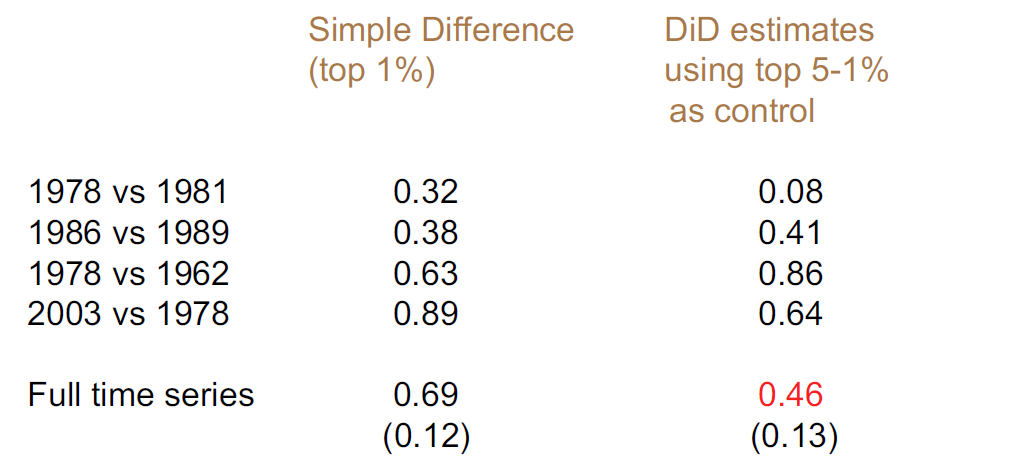
\includegraphics[width=4.5in]{images/ch13/13_DID_3.png}
                    \caption{Estimated Taxable Income Elasticity at the Top in the UK}
                \end{figure}

                With updated data, the estimate remains in the 0.35-0.55 range with \empha{a centre at 0.46}, but the standard error is high.

                Meanwhile, be aware that DiD method may have various problems here. For example, there is a key relationship between the size of elasticity and the tax base (\cite{slemrod_optimal_2002}), and there may be adjustment frictions.

        \subsection{Bunching Approaches}

            \subsubsection{Introduction}

                There is one important source of identification "neglected" in early studies: when there are kinks in the budget constraint, people bunch due to the discontinuous changes in the return to work.

                With certain assumptions, we can use non-parametric methods to retrieve a "local" elasticity from the mass at the bunching point.

                Throughout the bunching section, we denote the taxable income elasticity as $\epsilon$.

            \subsubsection{Bunching at Kink Points}

                \begin{figure}[H]
                    \centering
                    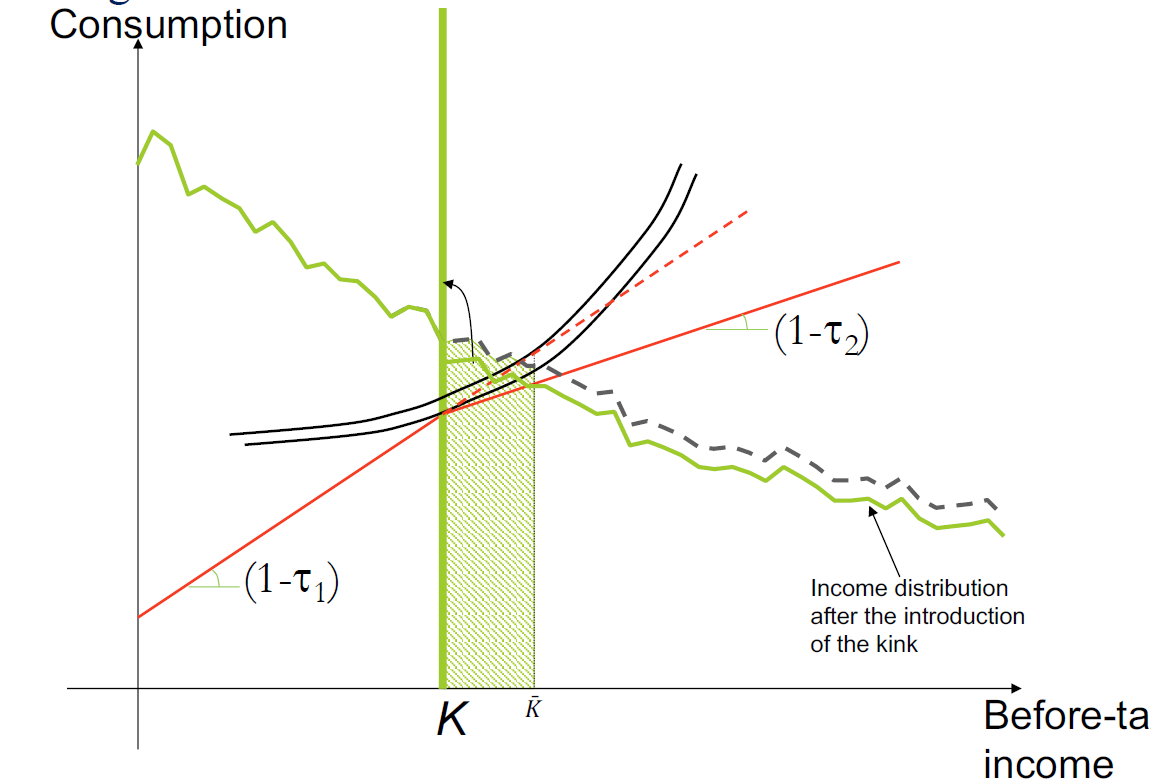
\includegraphics[width=0.49\textwidth]{images/ch13/13_bunching_1.png}
                    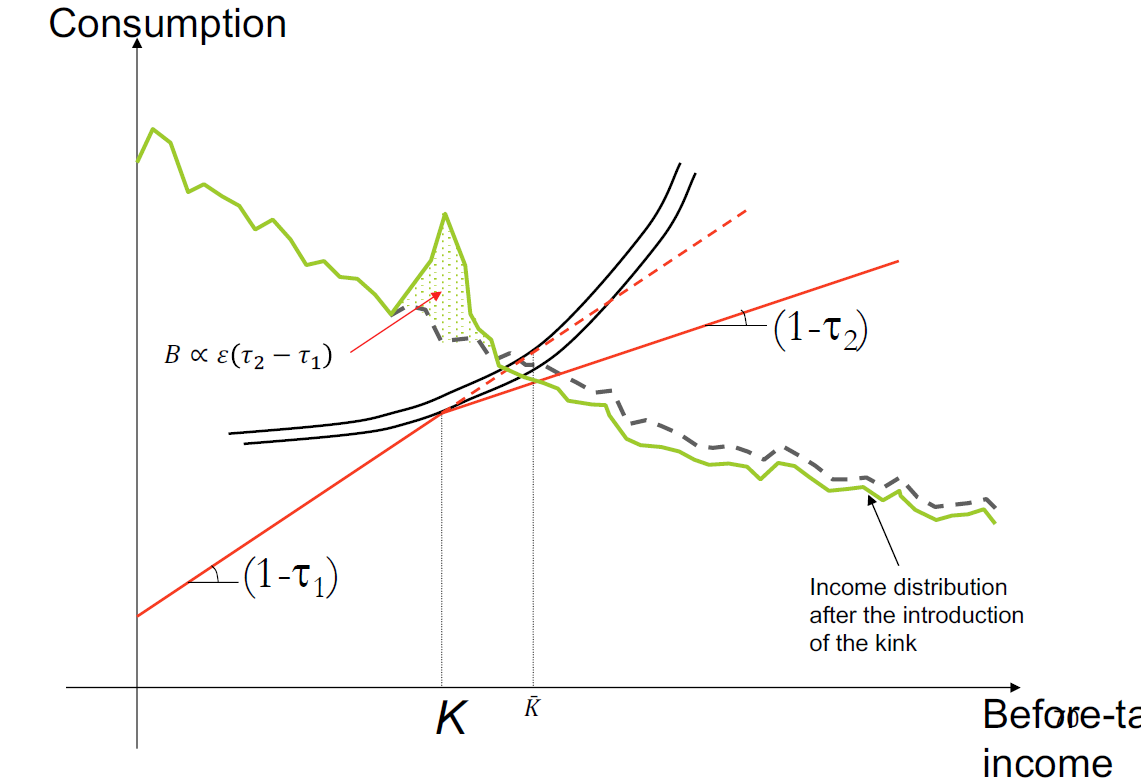
\includegraphics[width=0.49\textwidth]{images/ch13/13_bunching_2.png}
                    \caption{Bunching at Kink Points}
                \end{figure}


                \begin{figure}[H]
                    \centering
                    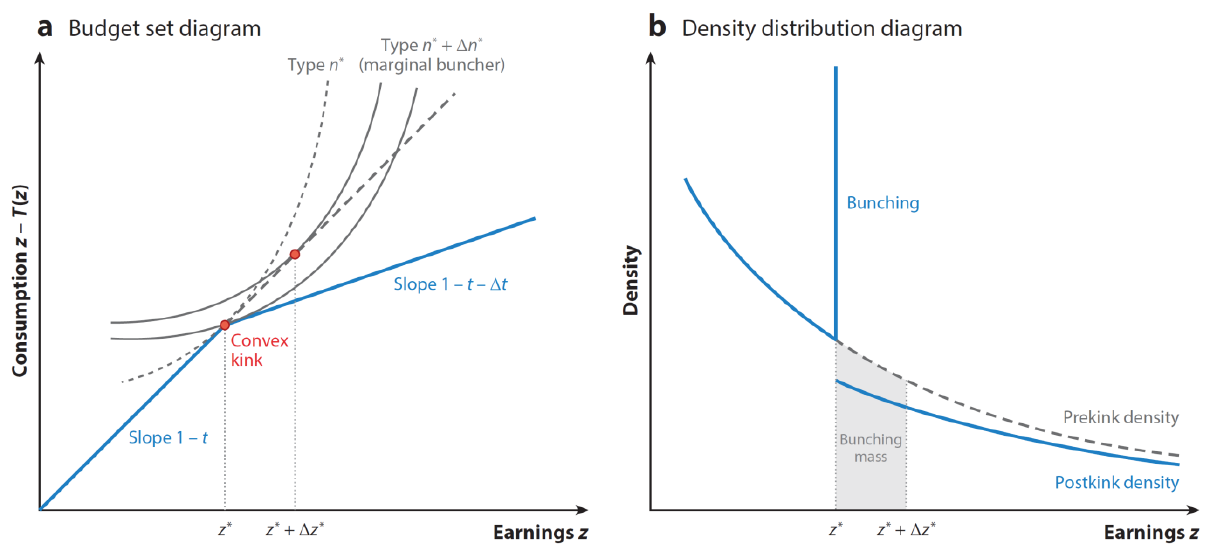
\includegraphics[width=5in]{images/ch13/13_bunching_3.png}
                    \caption{Bunching at Kink Points - Another Illustration}
                \end{figure}

            \subsubsection{Bunching Calculations: Start from Simple Single Upper Tax Bracket}

                The individual's optimisation problem is:
                $$
                \max c - \frac{\alpha}{1+\frac{1}{\epsilon}} \cdot \left( \frac{e}{\alpha} \right)^{1+\frac{1}{\epsilon}} \text{ s.t. } c \leq (1-\tau_1)e
                $$

                where $e=wh$ represents earnings and $\epsilon$ represents elasticity.

                Solving this optimisation, we can obtain the expression for optimal earnings:

                \begin{equation*}
                    e^\ast = \alpha (1-\tau_1)^\epsilon
                \end{equation*}
                
            \subsubsection{Bunching Calculations: Generalise to Several Brackets}

                We can then generalise our calculation to multiple tax brackets.

                Solving the optimisations, we can derive the range of earnings (if there were no kink) where individuals will move to the kink point:

                \begin{equation}
                    k \leq e^\ast \leq k \left( \frac{1-\tau_1}{1-\tau_2} \right)^\epsilon = \overline{k}
                    \label{eqn:bunching_1}
                \end{equation}

                where $k$ is the level of earning where MTR changes (the kink point).

            \subsubsection{Bunching Calculations: Mass of Bunches}

                From equation \ref{eqn:bunching_1}, we can calculate the mass at the bunching point:

                \begin{align*}
                    B &= \int_{k}^{\overline{k}} f(e^\ast) de^\ast \\
                    &\approx \frac{f(k)+f(\overline{k})}{2} \cdot (\overline{k}-k) \\
                    &= \frac{f(k)+f(\overline{k})}{2} \cdot k \cdot \left( \left( \frac{1-\tau_1}{1-\tau_2} \right)^\epsilon - 1 \right)
                \end{align*}

                Then, using the approximation $f(k) \approx f(\overline{k})$ around $k$ and the log approximation, we get the final bunch mass equation for our estimation:

                \begin{equation}
                    \color{red}
                    B \approx k\cdot f(k) \cdot \epsilon \cdot (\tau_2 - \tau_1)
                    \label{eqn:bunching_final}
                \end{equation}

                We can retrieve an estimate of $\epsilon$ by combining estimated mass $B$, estimated/extrapolated distribution $f(k)$, and institutional parameters $\tau_2,\tau_1,k$.

            \subsubsection{Bunching: Issues and Extensions}

                In equation \ref{eqn:bunching_final}, the estimates of $B,f(k)$ are sensitive to our assumptions. In reality, motivating our assumptions could be hard because MTRs vary by sources of taxable income as well as income level, and they have different elasticities.

                \begin{figure}[H]
                    \centering
                    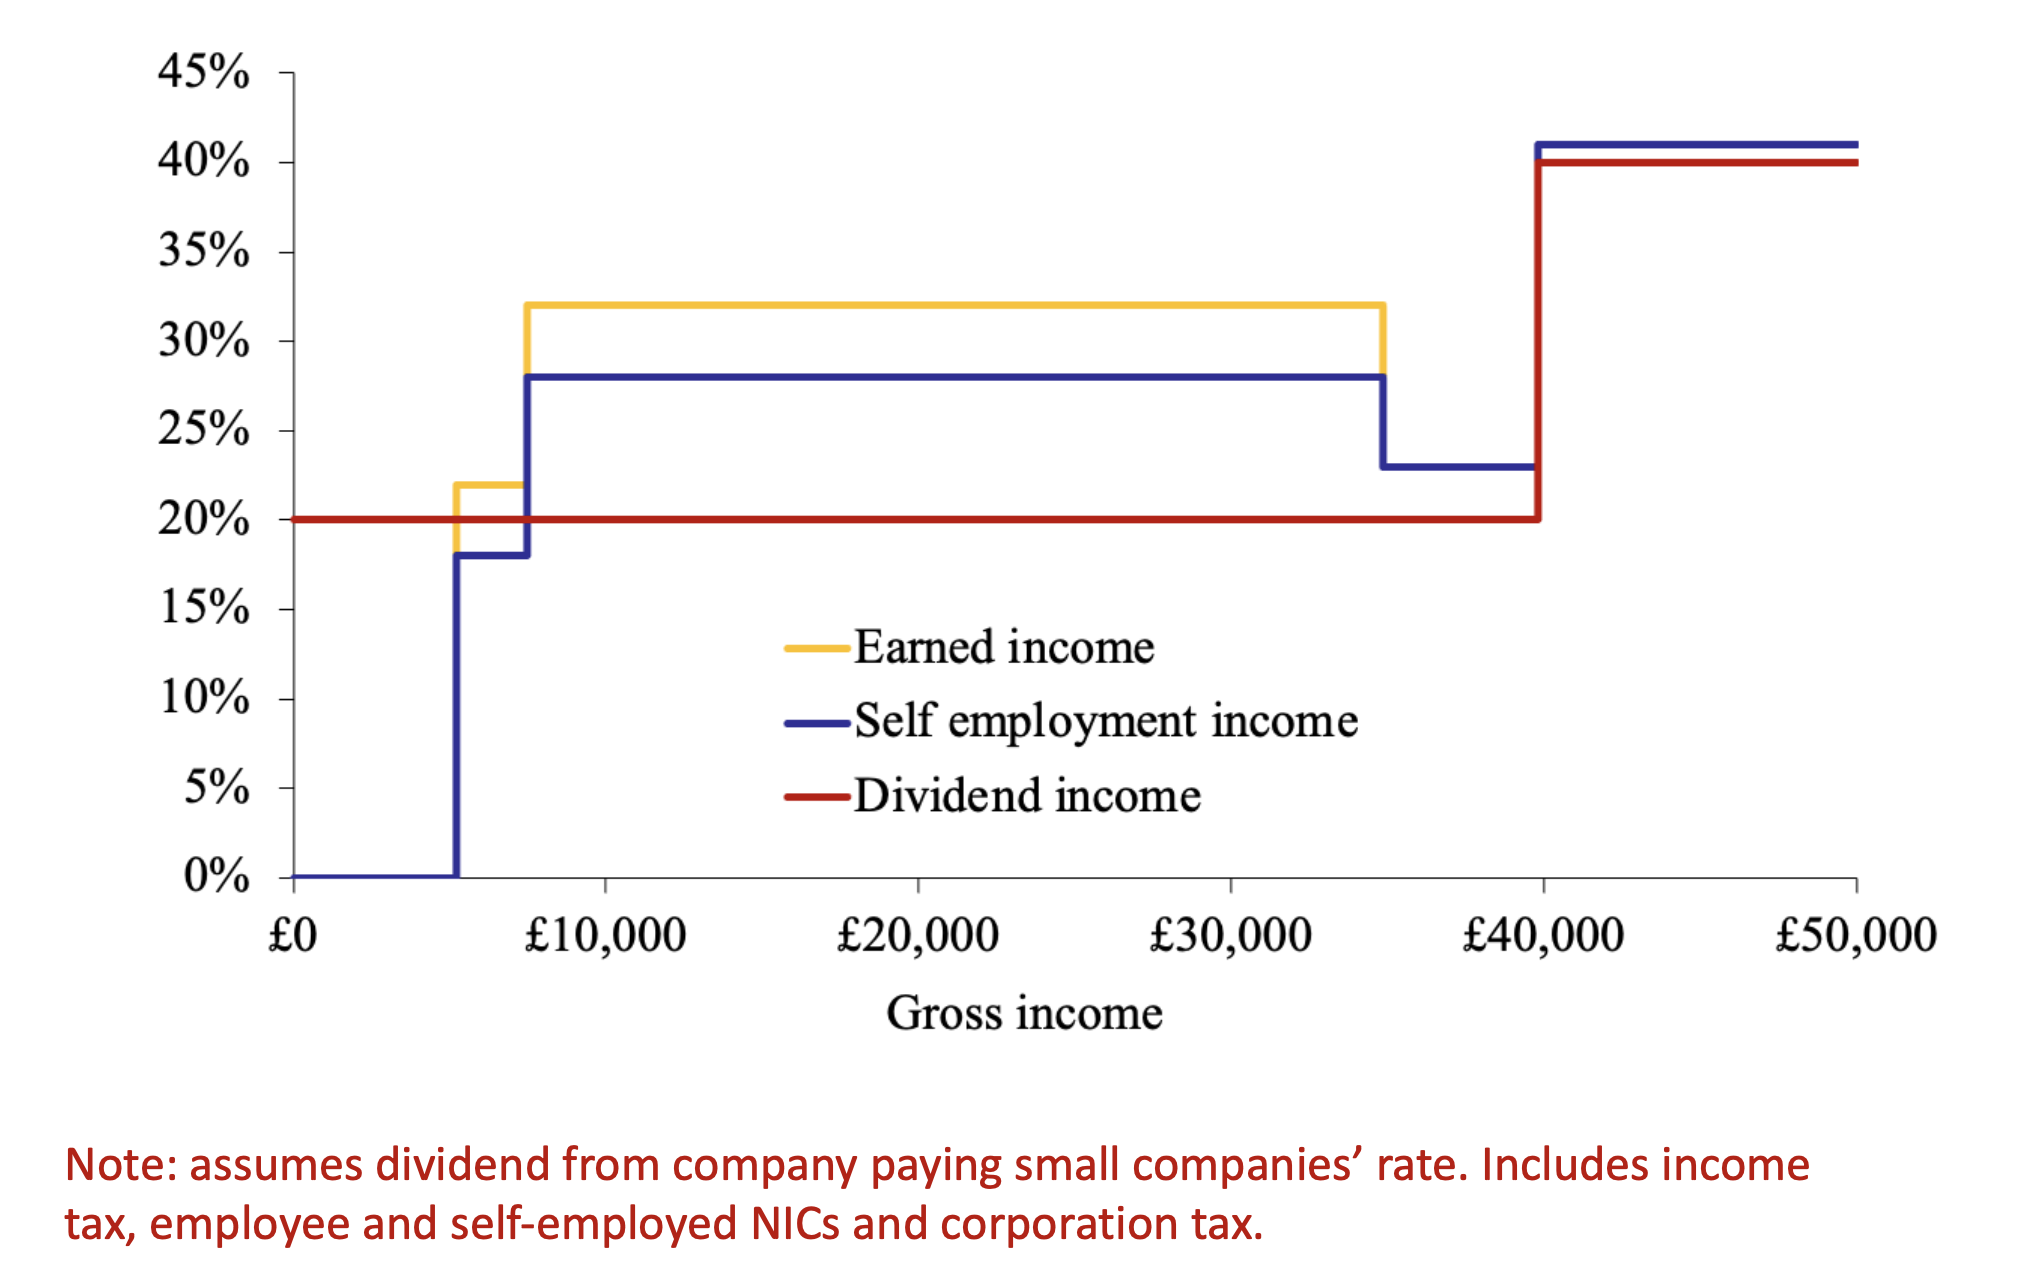
\includegraphics[width=4.5in]{images/ch13/13_bunching_4.png}
                    \caption{MTR of Different Sources of Incomes}
                \end{figure}

                \begin{figure}[H]
                    \centering
                    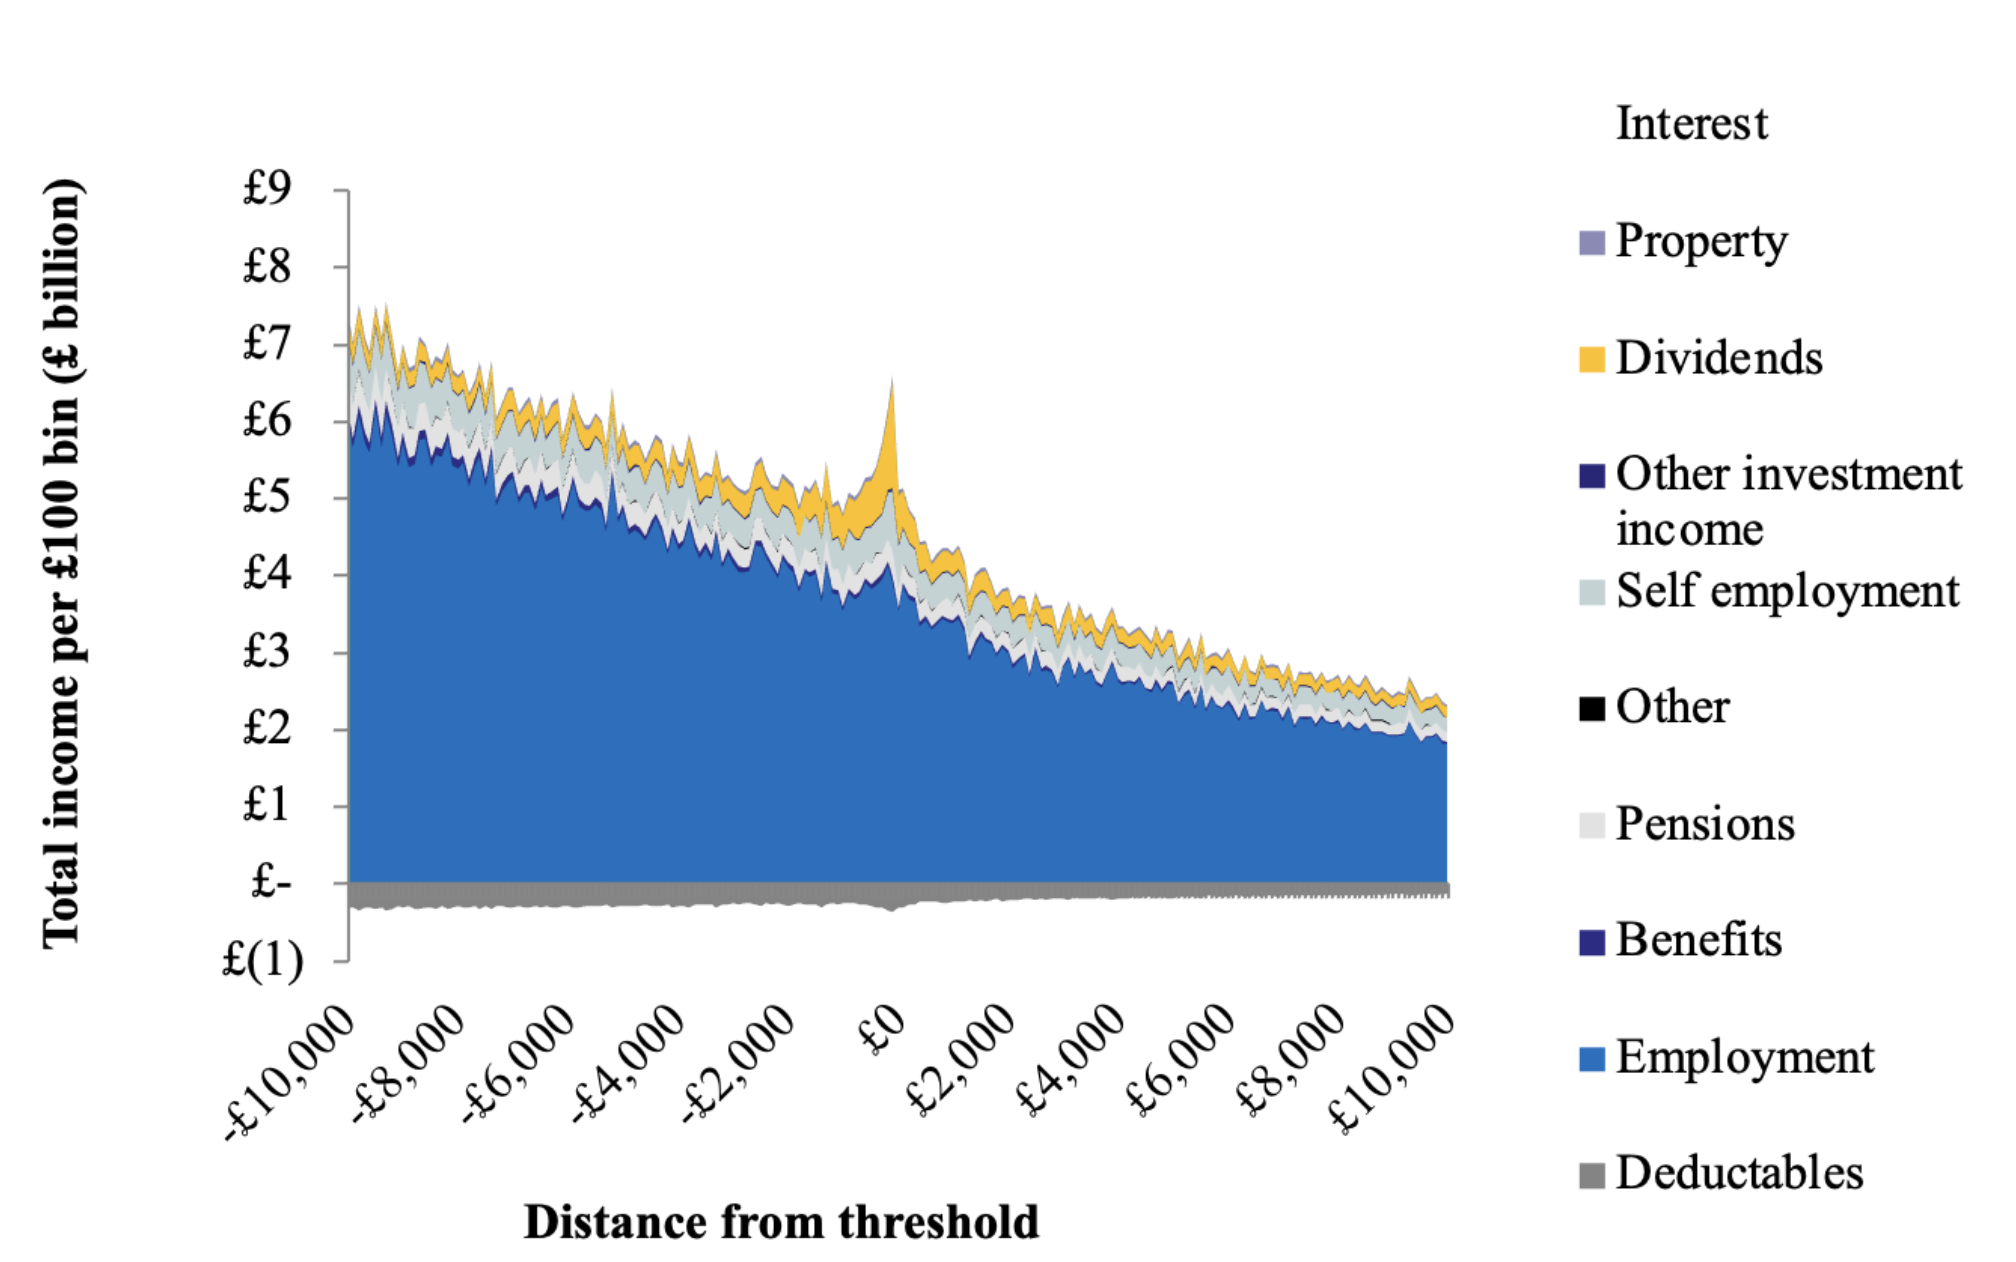
\includegraphics[width=4.5in]{images/ch13/13_bunching_5.png}
                    \caption{Different Sources of Incomes Have Different Elasticities}
                \end{figure}


    \subsection{Discussions and Extensions}

        Here are some possible topics for discussion:
        \begin{itemize}
            \item Has the taxable income elasticity $e$ changed over time?
            \item Is the method for estimating $e$ reliable?
            \item Is Pareto distribution assumption a good one? (Probably yes)
            \item How would a bargaining model change the arguments? With higher top tax rate $\tau$, the top income earners (usually business owners) may gain additional bargaining power over low-earning workers (\cite{piketty_optimal_2014}).
        \end{itemize}


\section{$\star$ The General Tax Schedule}

    \subsection{Introduction}

        The framework of optimal MTR discussed in section \ref{sec:optimal_top_tax} can be generalised to other income earners. At optimum,the costs and benefits of a small change in MTR are always balanced.

    \subsection{Three Impacts on Social Welfare}

        \subsubsection{Setup}
        
        Notations:

        \begin{itemize}
            \item For income $z$:
            \begin{itemize}
                \item $H(z)$ is the cumulative distribution (CDF) of individuals
                \item $h(z)$ is the density (PDF) of individuals
            \end{itemize}
            \item Total tax function $T(z)$ depends on income:
            \begin{itemize}
                \item There is a lumpsum grant $T(0)$
                \item Combined with a schedule of MTR $T'(z)=\frac{dT(z)}{dz}$
            \end{itemize}
            \item Consider a reform that changes the MTR $T'(z)$ by $d\tau$ in a small band of income ($z,z+dz$)
        \end{itemize}

        As in subsection \ref{sec:optimal_top_tax_impacts}, there will always be three impacts of a small change in MTR.
        
        \subsubsection{Mechanical Effect on Tax Revenue ($dM$)}

            With no behaviour response, an increase of the top rate will increase government revenue. This is beneficial to society, as the revenue can be used for government spending or higher transfers.

            Mathematically:

            \begin{equation}
                dM = (1-H(z)) \cdot dz \cdot d\tau
                \label{eqn:tax_gen_TR}
            \end{equation}

        \subsubsection{Behaviour Response on Tax Revenue ($dB$)}

            Again, higher MTR acts disincentive to working -- people may work less (substitution effect) and their taxable incomes will drop. This is a cost to society since tax revenue will decrease.

            This behavioural effect depends on the \emphb{elasticity of earnings with respect to the net of tax rate ($1-\tau$)}. For each individual, the change in MTR ($d\tau$) changes the earning by:

            \begin{equation*}
                dz = -e \cdot z \cdot \frac{d\tau}{1-T'(z)}
            \end{equation*}

            Since there are $h(z)dz$ such taxpayers, tax revenue will be reduced by:

            \begin{equation}
                dB = - h(z) \cdot dz \cdot e \cdot z \cdot d\tau \cdot \frac{T'(z)}{1-T'(z)}
                \label{eqn:tax_gen_BR}
            \end{equation}

        \subsubsection{Welfare Effect ($dW$)}

            Extra taxes also generate a welfare cost.

            Let $G(z)$ be the \emphb{average social value of distributing \textsterling 1 uniformly from taxpayers with income above $z$ (marginal value placed on income for individuals whose incomes are above $z$)}. The welfare effect is:

            \begin{equation}
                dW = - dM \cdot G(z)
                \label{eqn:tax_gen_WE}
            \end{equation}

            Note that the "welfare cost" will have the opposite sign.

    \subsection{The Choice of the Top Tax Rate}
    
        \subsubsection{Optimum}

            Summing up the three effects (equation \ref{eqn:tax_gen_TR}, \ref{eqn:tax_gen_BR}, and \ref{eqn:tax_gen_WE}). The overall effect of a small change in top rate ($d\tau$) is:
    
            \begin{equation*}
                dM + dB + dW = \Big\{ (1-G(z)) \cdot (1-H(z)) \cdot dz \cdot d\tau \Big\} - \Big\{ h(z) \cdot dz \cdot e \cdot z \cdot d\tau \cdot \frac{T'(z)}{1-T'(z)} \Big\}
            \end{equation*}
    
            At optimum, this has to be zero:
    
            \begin{equation*}
                dM + dB + dW = \Big\{ (1-G(z)) \cdot (1-H(z)) \cdot dz \cdot d\tau \Big\} - \Big\{ h(z) \cdot dz \cdot e \cdot z \cdot d\tau \cdot \frac{T'(z)}{1-T'(z)} \Big\} = 0
            \end{equation*}
    
            This can be simplified to:
    
            \textcolor{red}{\begin{align}
                \frac{T'(z)}{1-T'(z)} &= \frac{(1-G(z)) \cdot (1-H(z))}{e \cdot z \cdot h(z)} \\
                &= \frac{1}{e} \cdot \frac{1-H(z)}{h(z) \cdot z} \cdot (1-G(z))
            \end{align}}

        \subsubsection{Interpretation}

            We can see that:
            \begin{itemize}
                \item The optimal tax rate decreases with taxable income elasticity $e$
                \item The optimal tax rate decreases with $G(z)$ which measures the marginal value placed on income for individuals whose incomes are above $z$
                \item The optimal tax rate decreases with the hazard ratio $\frac{1-H(z)}{h(z) \cdot z}$, which measures the thinness of the distribution
            \end{itemize}

    \subsection{Extensions: Negative MTR and Extensive Margins}

        \subsubsection{Negative MTR?}

            In this framework \empha{with only intensive margins, negative MTRs are never optimal}: if the MTR were negative in some range, then increasing it a bit in that range would raise the tax revenue and decrease the net earnings of taxpayers in that range ($dB>0$). However, the behavioural response (working less) would also raise tax revenue as $MTR<0$ in that range. Therefore, a small tax increase will increase social welfare unambiguously, so optimum cannot be achieved as long as negative MTR exists.

            However, if we introduce the extensive margin / participation decision of labour supply, then this argument would change. (next)

        \subsubsection{Extensive Margins: Setup}

            Some additional setups:
            \begin{itemize}
                \item If an individual decides to work, he/she gets $z-T(z)$
                \item If he/she decides not to work, he/she gets $-T(0)$
                \item Suppose the utility function is linear: $u=c-q$
                \begin{itemize}
                    \item $c$ is disposable income
                    \item $q$ is the cost of work, distributed with CDF: $P(q|z)$
                \end{itemize}
                \item Define the \emphb{elasticity of participation (extensive margin elasticity) $\eta$} as $$\eta = \frac{z-T(z)+T(0)}{P} \cdot \frac{\partial P}{\partial q}$$
                \item Allow MTR to be different across $I$ earning groups indicated by $i$
            \end{itemize}

        \subsubsection{Extensive Margins: Optimum and Interpretations}

            With extensive margins, the formula for optimal taxes will be:
            
            \begin{equation}
                \color{red}
                \frac{T_i - T_{i-1}}{c_i - c_{i-1}} = \frac{1}{e_i h_i} \sum_{j\geq 1}^I \left[ 1 - g_j -\eta_j \cdot \frac{T_j - T_0}{c_j - c_0} \right]
            \end{equation}
            
            Literature on labour supply suggests that \empha{extensive margin is more responsive than intensive margin. At the bottom of the income distribution, high MTRs are not necessarily desirable and negative participation tax rates could be optimal. }

        